%% Copernicus Publications Manuscript Preparation Template for LaTeX Submissions
%% ---------------------------------
%% This template should be used for copernicus.cls
%% The class file and some style files are bundled in the Copernicus Latex Package, which can be downloaded from the different journal webpages.
%% For further assistance please contact Copernicus Publications at: production@copernicus.org
%% http://publications.copernicus.org/for_authors/manuscript_preparation.html
%% Please use the following documentclass and journal abbreviations for discussion papers and final revised papers.
%% 2-column papers and discussion papers
\documentclass[journal abbreviation, manuscript]{copernicus}
%% Journal abbreviations (please use the same for discussion papers and final revised papers)
% Archives Animal Breeding (aab)
% Atmospheric Chemistry and Physics (acp)
% Advances in Geosciences (adgeo)
% Advances in Statistical Climatology, Meteorology and Oceanography (ascmo)
% Annales Geophysicae (angeo)
% ASTRA Proceedings (ap)
% Atmospheric Measurement Techniques (amt)
% Advances in Radio Science (ars)
% Advances in Science and Research (asr)
% Biogeosciences (bg)
% Climate of the Past (cp)
% Drinking Water Engineering and Science (dwes)
% Earth System Dynamics (esd)
% Earth Surface Dynamics (esurf)
% Earth System Science Data (essd)
% Fossil Record (fr)
% Geographica Helvetica (gh)
% Geoscientific Instrumentation, Methods and Data Systems (gi)
% Geoscientific Model Development (gmd)
% Geothermal Energy Science (gtes)
% Hydrology and Earth System Sciences (hess)
% History of Geo- and Space Sciences (hgss)
% Journal of Sensors and Sensor Systems (jsss)
% Mechanical Sciences (ms)
% Natural Hazards and Earth System Sciences (nhess)
% Nonlinear Processes in Geophysics (npg)
% Ocean Science (os)
% Proceedings of the International Association of Hydrological Sciences (piahs)
% Primate Biology (pb)
% Scientific Drilling (sd)
% SOIL (soil)
% Solid Earth (se)
% The Cryosphere (tc)
% Web Ecology (we)
% Wind Energy Science (wes)
%% \usepackage commands included in the copernicus.cls:
%\usepackage[german, english]{babel}
%\usepackage{tabularx}
%\usepackage{cancel}
%\usepackage{multirow}
%\usepackage{supertabular}
%\usepackage{algorithmic}
%\usepackage{algorithm}
%\usepackage{amsthm}
%\usepackage{float}
%\usepackage{subfig}
%\usepackage{rotating}
\begin{document}
\title{Plume-SPH 1.0: A 3D dust-gas volcano plume model based on smoothed particle hydrodynamics}
% \Author[affil]{given_name}{surname}
\Author[1]{Zhixuan}{Cao}
\Author[1]{Abani}{Patra}
\Author[2]{Marcus}{Bursik}
\Author[3]{E. Bruce}{Pitman}
\Author[4]{Matthew}{Jones}
\affil[1]{Department of Mechanical and Aerospace Engineering, University at Buffalo, SUNY, New York, United State}
\affil[2]{Department of Geology, University at Buffalo, SUNY, New York, United State}
\affil[3]{Department of Mathematics, University at Buffalo, SUNY, New York, United State}
\affil[4]{Center for Computational Research,
University at Buffalo, SUNY, New York, United State}
%% The [] brackets identify the author with the corresponding affiliation. 1, 2, 3, etc. should be inserted.
\runningtitle{Plume-SPH 1.0}
\runningauthor{Z. Cao et al}
\correspondence{Abani Patra (abani.patra@gmail.com)}
\received{}
\pubdiscuss{} %% only important for two-stage journals
\revised{}
\accepted{}
\published{}
%% These dates will be inserted by Copernicus Publications during the typesetting process.
\firstpage{1}
\maketitle
\begin{abstract}
Volcanic ash, if persists in the atmosphere, will pose great threat on aircrafts and communities. VATDs (Volcanic ash transport and dispersion models) usually take output of plume models as source terms. The accuracy of source terms is crucial for VATDs. All of existing 3D (three dimensional) plume models are using mesh-based methods. SPH (Smoothed particle hydrodynamics), as a mesh free method has several advantages over mesh-based methods in modeling of multiphase free boundary flow. As an initial effort on exploiting the feasibility and advantage of SPH in volcano plume modeling we adopt a relative simpler model, a 3D dusty-gas dynamic model, targeting at capturing the more basic features of volcano plume. In this model, erupted material is assumed to be well mixed and represented by one phase while air is another phase. Immediate dynamic and thermal dynamic equilibrium between air and erupted material are assumed. Affect of wind is not considered. Several newly developed techniques in SPH are adopted and trimmed to address numerical challenges in simulating multiphase compressible turbulent flow with classical SPH method. The $SPH-\varepsilon$ turbulence model is adopted to capture sub-particle mixing. Heat exchange due to turbulence is then calculated with Reynolds analogy. Corrected formulism of SPH is used to handle tensile instability and deficiency of particle distribution near the boundaries. We also propose feasible ways to impose velocity inlet and pressure outlet boundary conditions, both of which are scarce in traditional implementation of SPH. Core solver of our model is parallelized with MPI (message passing interface) obtaining good weak scalability and strong scalability. The model is first verified by comparing velocity and concentration distribution along axis and cross section with experimental results of JPUE (jet or plume which is ejected from a nozzle into a uniform environment). The top height of Pinatubo eruption (15 June 1991) simulated by our model is consistent with both observation and existing 3D plume models. Profiles of several integrated variables are compared with these by existing 3D plum models and further verifies the correctness of our model. Analysis on the plume evolution process illustrated that this model is able to reproduce the basic physics of plume development. The comparison also implies that turbulence model plays a significant role in 3D volcano plume modeling.
\end{abstract}
\introduction  %% \introduction[modified heading if necessary]
\subsection{Volcanic ash hazards}
The dynamics of explosive eruption clouds has been the central issue of volcanology science for a long time. Primary hazards associated with explosive grey volcanoes include pyroclastic density currents (flows and surges), the widespread deposition of airfall tephra, and the threats posed by volcanic ash. In addition, there are also other secondary hazards associated with volcanoes \citep{lockwood2013volcanoes}.
Simulation of all possible hazards with one model is difficult due to diversity among these hazards. Our concern in current work is the risks that volcanic ash posed on aircrafts and communities. During volcanic eruptions, VATDs (volcanic ash transport and dispersion models) are used to forecast the location and movement of ash clouds over hours to days. Those VATDs use eruption source parameters, such as plume height, mass eruption rate, duration, and the mass fraction distribution of erupted debris finer than about $4 \Phi$ (or $63  \mu$m), which can remain in the cloud for many hours or days. Observational data for such parameters are usually unavailable in the first minutes or hours after an eruption is detected. Moreover, these input parameters are subject to change during an eruption, requiring rapid re-assignment of new parameters. Usually, plume models are used to provide sources terms for VATDs. This paper reports a new 3D (three dimensional) volcano plume model exploiting advantage of mesh-free methods in multiple phase free boundary flow modeling.\\
%
\subsection{Existing plume models}
The basic physics behind of volcanic plume has been understood for more than half a century \citep{morton1956turbulent, settle1978volcanic, wilson1978control}. Several volcano plume models have been developed in the past few decades. Specific aspects of a plume have been studied by 1D (one dimensional) plume models which describe the steady state solution of a plume under idealized boundary conditions.
The effects of magma type and vent conditions \citep{woods1988fluid, woods1995decompression}, atmospheric conditions \citep{ woods1993moist, sparks1997volcanic, bursik2001effect}, external surface water \citep{koyaguchi1996formation}, thermal disequilibrium, and particle fallout \citep{woods1991particle} have been assessed in increasing details through 1D numerical simulations. Recently developed 1D models (eg. \citep{mastin2007user, woodhouse2013interaction}) tend to accounting for more physics effects in one model. FPLUME-1.0 \citep{folch2016fplume} accounts for wind affect, entrainment of moisture, water phase change, particle fallout and re-entrainment and even wet aggregation of ash. However, In these 1D models, the entrainment of air is evaluated based two coefficients: entrainment coefficient for the vertical plume and the entrainment coefficient that describes the effect of wind. Different 1D models adopt different entrainment coefficients based on specific formulation or calibration against well-documented case studies. The feedback from plume to atmosphere is ignored in 1D models. Even though determination of essential parameters such as the entrainment is not based on first principles, such simple models nevertheless allow us to investigate the importance of physical mechanisms in a volcanic plume. In addition, these simplified models requires little computational sources and can run on standard personal computers or on web sites in very short time. As a result, 1D software (such as \citep{267, 1194, 3541}) for volcano plume development, combined with VATDs (such as \citep{114, draxler2015hysplit}) are widely used in research and practice. While these 1D models can generate well-matched results with 3D (three dimensional) models for weak plumes, much greater variability is observed for strong plume scenarios, especially for local variables \citep{costa2016results}. In addition, the need for greater skills in associated hazards forecasts with 1D models requires 2D (two dimensional) and 3D models.\\
The development of 2D and 3D, time-dependent, and multiphase numerical models for volcano plume has provided new explanations for many features of explosive volcanism. One of these 3D models is PDAC (Pyroclastic Dispersion Analysis Code) \citep{neri2003multiparticle}  which is a non-equilibrium, multiphase, 3D compressible flow model. Conservation equations for each phase are solved separately with finite volume method. And a parallel computing version of PDAC was developed lately \citep{ongaro2007parallel}. Advanced numerical techniques, such as second order scheme and semi-explicit time upgrading, was also adopted afterwards to improve the accuracy of PDAC \citep{carcano2013semi}. 
Another 3D model, SK-3D \citep{suzuki2005numerical} is a three-dimensional time-dependent fluid dynamics model that can reproduce the entrainment process of eruption clouds with relative simpler physics but high order of accuracy and high spatial resolution, which is applicable to time-dependent phenomena in actual volcanological simulations. 
A serials of simulations based on SK-3D was conducted, including determination of the entrainment coefficients of eruption columns as a function of height \citep{suzuki2010numerical}, study the effect of wind field on entrainment coefficient \citep{suzuki20133d}, establishment of the relationship between the observable quantities of the eruption clouds and the eruption conditions at the vent \citep{suzuki2009three} (previously, such relationship is based on 1D models and greatly depends on empirical constants), investigation of the effect of the intensity of turbulence in the umbrella cloud on dispersion and sedimentation of tephra \citep{koyaguchi2009effect}. 
While the SK-3D focuses on accurately capturing the entrainment caused by turbulent mixture with higher resolution and numerical method of higher order, PADC takes the disequilibrium between different phases into account and hence is a true multiphase model. Another 3D model, ATHAM ( Active Tracer High-Resolution Atmospheric Model) \citep{oberhuber1998volcanic} focuses more on microphysics within the plume. As pyroclastic flow is not the initial concern of ATHAM, immediately dynamics and thermodynamics equilibrium is assumed in ATHAM. The dynamic core of ATHAM solves the compressible Euler equations for momentum, pressure and temperature of the gas particle mixture \citep{oberhuber1998volcanic}. The subgrid-scale turbulence closure scheme differentiates between the horizontal and vertical directions \citep{herzog2003prognostic} to capture turbulent mixing. The cloud microphysics predicts the mass of hydrometeors in liquid and ice phase \citep{herzog1998effect}. Additional modules include radiation \citep{langmann1997radiative}, gas phase chemistry \citep{trentmann2002simulation} and gas scavenging by hydrometeors \citep{textor2003injection} were added lately. An further extension was made to include particle aggregation in 2006 \citep{textor2006volcanic1, textor2006volcanic2}. However, the resolution of ATHAM is still pretty coarse compared with SK-3D and PDAC.
Besides strengthening their strength (ATHAM has been adding more and more microphysics, PDAC was extended to consider more phases), these models are learning from each other. PDAC is trying to include effect of microphysics into the model while ATHAM wants to extend its ability to modeling pyroclastic flow. Both are using finer and finer resolution. Recently, A first order, non-equilibrium compressible 3D model, ASHEE \citep{cerminara2016ashee}, is derived based on three dimensional N phases Eulerian transportation equation. ASHEE is valid for low concentration and low Strokes number region and much faster than N-phase Eulerian model. The model is based an open source numerical solver OpenFOAM adopting unstructured finite volume method.\\
To summarize, each model has its own focus based on problem of interest. Different simplification was made based on their scope. Improvements have been making since their birth. Accuracy (depends on comprehensiveness of the model, resolution of discretization, numerical error, and order of accuracy) and simulation time (depends on number of governing equations, resolution, numerical methods and parallel techniques) are always a couple of conflict considerations in 3D plume simulations.\\
%
\subsection{Features of SPH}
All of these existing 3D models are based on mesh-based methods (Eulerian methods). And there is no 3D plume model based on mesh free method (Lagrange methods) yet. Actually, Lagrangian methods have several features that are suitable for volcano plume simulation. Among such Lagrangian methods, Smoothed Particle Hydrodynamics \citep{gingold1977smoothed,lucy1977numerical}, even though relatively newer compared to well designed mesh based methods such as Finite Difference, has shown good agreement with experiments by many applications in fluid dynamic area. And it currently is, by far the most widely used scheme. Specifically, the reason we choose SPH as the numerical method for volcanic plume simulation are as following:
\begin{itemize}
\item For mesh based method, either interface tracking (Lagrangian) \citep{harlow1965numerical, wrobel1991computational, cheng1995simplified} or interface capturing (Eulerian) \citep{hirt1981volume, youngs1982time, gerlach2006comparison, gopala2008volume} methods are used to reconstruct the flow interface of free boundary flow. High computational cost, a tendency to form numerical instabilities and the inability to track complex topological changes are the significant drawbacks of Lagrangian techniques \citep{hirt1981volume, unverdi1992front, anderson1998diffuse}. For interface capturing (Eulerian) method, the surrendering of surface detail before the phase transport calculation means that interface reconstruction is required between time steps to recover the interface information, which need additional numerical effort \citep{hirt1981volume, youngs1982time}. Being able to adaptively adjust the discretization and automatically construct the interface, SPH does not require additional numerical effort for interface construction and therefor more suitable for volcano plume simulation.
\item Advection term in the Navier-Stokes equations does not appear explicitly in discretized formula of SPH (as illustrated in Eq. (\ref{eq:gov-nc-rho}) to Eq. (\ref{eq:gov-nc-e})). So advection term will be treated exactly with SPH \citep{monaghan2005smoothed}.
\item It is easy to include various physics effect (like self gravity, radiative cooling and chemical reaction) into the model. It does not require a major overhaul and re-tooling every time new physics is introduced \citep{monaghan1995sph}. This implies that accounting for more physics is easier for SPH model.
\item With more than one material, each described by its own set of particles, interface problems between phases are often trivial for SPH but difficult for mesh based schemes. So multiple phase flow can be easily handled by SPH. Adding of new phases to the model also does not require a major overhaul and re-tooling. As will be shown in later paragraph, adding of new phases will lead to adding of several lines into the source code for new phases and additional interaction terms between existing phases and newly added phases.
\end{itemize}
As discussed in the previous paragraph, existing 3D plume models focus on one or several specific aspects of plume and have been extended to be more comprehensive by accounting for more physics or more phases. Easy extensibility and capability of handling multiples phase flow without additional numerical effort greatly facilitate future extension of SPH models. As volcanic plume are in nature multiphase and without pre-defined boundary in the atmosphere, SPH is a suitable numerical method for plume modeling. The more basic physics, such as entrainment of air and thermal expansion, are essential for all plume modeling while some other physics, such as water condense and aggregation ect., are important in specific scenario. As an initial effort on exploiting advantages of SPH in volcano plume modeling, we focus on capturing more basic features in plume development. So our current model is far away from comprehensive. Fortunately, the easy extension feature of SPH facilitate developing of a more comprehensive model in the future.\\
%
\subsection{Our contribution}
As SPH is a relative new method in computational fluid dynamics, implementation of SPH for compressible multiphase turbulent flow is scarce. Several remedies of classical SPH are adopted in our implementation. One of the most popular implementations of SPH is simulating of free surface flow, such as breaking-waves and flood. Less attention was paid to velocity inlet and pressure outlet boundary conditions which are required in plume modeling. We impose pressure boundary condition by adding extra layers of static ghost particles. Additional constrain on time step is used to avoid growing up of numerical fluctuations near the pressure boundary. We impose velocity inlet boundary condition by placing several layers of ghost particles moving with eruption velocity. Turbulence model is crucial for reproducing the entrainment of air. There are several turbulence models proposed for SPH method \citep{issa2005numerical,violeau2007numerical}. We adopt a LANS (Lagrangian Averaged Navier-Stokes) turbulence model \citep{monaghan2011turbulence}, which was originally proposed for incompressible, and extend it for compressible flow accounting for turbulent heat exchange. Corrected formulism of SPH is adopted to bypass the well-known tensile instability issues of classical SPH.\\
%
Simulation of volcano plume with acceptable accuracy requires fine resolutions (very high particle counts) that cannot be accomplished without parallel computing within given time window. The core solver of our model is parallelized by MPI (message passing interface standard) parallelism. In addition, a dynamic load balancing strategy is also developed. What's more, imposing of some types of boundary conditions (such as eruption boundary condition) requires dynamically adding and removing of particles during simulation. To address this issue, we adopt an efficient data management scheme based on time dependent SFC (space filling curve) and hash table. The computational cost is further reduced by adjusting simulation domain adaptively.\\
The organization of this paper is as following:
The physics model of the plume is first presented in section \ref{sec:physics-model} and leads to a complete mathematical description of the volcano plume (governing equations and boundary conditions). In section \ref{sec:SPH_method} we will briefly introduce the numerical tool, SPH method. Both the fundamental discretization formulism and techniques that used to handle specific issues involved in plume modeling will be discussed. Validation and verification with numerical tests is presented in section \ref{sec:verification-validation}. In section \ref{sec:conclusion}, a discussion on future work is given following a brief summary.
\section{Physical Model} \label{sec:physics-model}
\subsection{Description of the model}
During an explosive eruption, a volcanic jet erupts out from a vent with a speed of several tens to more than 150 meters per second, driven by expanding gas. The jet is initially denser than the surrounding atmosphere and begins to decelerate through negative buoyancy and turbulent interaction with surrounding air. Cauliflower-like vortices are generated along jet margins, within which process, air is entrained and heated up, reducing the bulk density of the entire jet, in many cases, to less than that of the surrounding atmosphere. Once it becomes buoyant, such a jet develops into a plinian or subplinian plume, rising kilometers to tens of kilometers until its heat is exhausted that buoyancy is lost. Jets that lose their momentum before becoming buoyant collapse back onto the ground and transform into pyroclastic flows, surges and ignimbrites. Simutaneously, relative coarse particle might separate with main stream of the plume falling down onto the ground and may be re-entrained into the plume at a lower height \citep{ernst1996sedimentation}. Within this process, erupted vapor will condense to liquid (droplet) and even further to ice. Latent heat released from phase change of erupted vapor will further heat up entrained air and make the bulk density further dilute. Even entrained vapor might also experience similar process and impose impact on plume development. Particle aggregation process \citep{carey1982influence,taddeucci2011aggregation}, either due to presence of liquid water, resulting from particle collision or driven by electrostatic forces might occur inside plume and thereby affect the sedimentation. 
This is essentially a multiple phases turbulent mixing process coupled with heat transfer and many other microphysics. As an initial effort on exploiting the feasibility and advantage of SPH in plume modeling, our model is designed to describe an injection of well mixed solid and volcanic gas from a circular vent above a flat surface into a stratified stationary atmosphere following SK-3D \citep{suzuki2005numerical}. In this model, molecular viscosity and physics heat conduction is neglected since turbulent exchange coefficients are dominant. Erupted material consist of solid with different size and mixture of gases (various constituent) is assumed to be well mixed and behave like a single phase fluid (phase 2) which is valid for eruptions with fine particles and ash. Air (also a mixture of different gases) is assumed to be another phase (phase 1). Immediate thermodynamics equilibrium is assumed so that no separate energy equation is needed for each phase. As a result, there is only one energy equation for both phases (heat exchange term between different phases will not show up under this assumption). Immediate dynamics equilibrium is assumed so that no separate momentum equation is needed for each phase. As a result, there is only one vector momentum equation for both phases (drag force term will not show up with this assumption). Because of above assumptions, all other micro-physics process (like phase change of  \texorpdfstring{H\textsubscript{2}O}, aggregation, decomposition, absorption of gas on the surface of solid, solution of gas into the liquid) and chemical process will not be considered in this model. These microphysics factors will come to play critical roles under particular eruption conditions. Capturing of these processes need a more comprehensive model. One critical element in plume development, the affect of wind, is also not considered in this model yet. Introducing of wind effect in our model will need imposing of pressure boundary conditions in a dynamic way, which requires more numerical effort and algorithm design. To summarize, our model is not valid for eruptions where wind affect plays a significant role in its development, usually refereed as weak plume. Our model is also lack ability in modeling plumes with large particles or in which microphysics plays non-ignorable roles, such as a eruption of \textit{El Chich{\'o}n} volcano at April 4th \citep{sigurdsson19841982, folch2016fplume}. At present stage, we are more interested in more basic (and more critical) aspects of volcano plume and therefor devote our effort to this relative simpler model. It is worthwhile to mention here that because SPH is adopted as our numerical method, adding of these physics into our model would require much less work in terms of programming compared to mesh based methods.\\
\subsection{Governing equations}
Based above assumptions, the governing equation of our model is given as following, which is the same as governing equations of SK-3D \citep{suzuki2005numerical}.
\begin{align}
\dfrac{\partial \rho}{\partial t} + \nabla \cdot (\rho \textbf{v}) = 0 \label{eq:gov-cs-rho} \\
\dfrac{\partial \rho \xi}{\partial t} + \nabla \cdot (\rho \xi \textbf{v}) = 0 \label{eq:gov-cs-ks}\\
\dfrac{\partial \rho \textbf{v}}{\partial t} + \nabla \cdot (\rho \textbf{v} \textbf{v} + p\textbf{I}) = \rho \textbf{g} \label{eq:gov-cs-v} \\
\dfrac{\partial \rho E}{\partial t} + \nabla \cdot [(\rho E + p )\textbf{v}] = \rho \textbf{g} \cdot\textbf{v} \label{eq:gov-cs-e}
\end{align}
$\xi$ is the mass fraction of ejected material.
$E = e + K $ is total energy which is summation of kinetic energy $K$ and internal energy $e$.
An additional equation is required to close the system. In this model, the equation for closing the system is the EOS (equation of state) for ideal gas.
\begin{equation}
p = (\gamma_m - 1)\rho e \label{eq:EOS}
\end{equation}
Where 
\begin{equation}
\gamma_m = R_m/C_{vm} + 1 \label{eq:gov-gm}
\end{equation}
\begin{equation}
R_m = n_gR_g + n_aR_a  \label{eq:gov-Rm}
\end{equation}
\begin{equation}
C_{vm} = n_s C_{vs} + n_g C_{vg} + n_a C_{va} \label{eq:gov-Cvm}
\end{equation}
\begin{equation}
n_a = 1 - \xi \label{eq:gov-na}
\end{equation}
\begin{equation}
n_g = \xi n_{g0} \label{eq:gov-ng}
\end{equation}
\begin{equation}
n_s = \xi - n_g \label{eq:gov-ns}
\end{equation}
Where, $C_v$ is specific heat with constant volume, $n$ is mass fraction, $R$ is gas constant. The subscript 
$m$ represents mixture of ejected material and air, $s$ represents solid portion in ejected material, $g$ represents gas portion in the ejected material and $a$ represents air.
In mesh based method, governing equations in Eulerian form, Eq. (\ref{eq:gov-cs-rho}) to Eq. (\ref{eq:gov-cs-e}), will be directly discretized. For SPH, governing equations in Lagrange form is needed. By deducting Kinetic energy from energy equation, subtracting mass conservation from momentum equation, combining transient term and advection term into material derivative term, the governing equation is put into the final formulism, in which advection term does not show up explicitly.
\begin{align}
\dfrac{D \rho}{D t} + \rho \nabla \cdot \textbf{v} = 0 \label{eq:gov-nc-rho}\\
\dfrac{D \rho \xi}{D t} + \rho \xi \nabla \cdot \textbf{v} = 0 \label{eq:gov-nc-ks}\\
\dfrac{D \textbf{v}}{D t} + \dfrac{\nabla P}{\rho} =\textbf{g} \label{eq:gov-nc-v}\\
\dfrac{D e}{D t} + \dfrac{P \nabla \cdot \textbf{v}}{\rho} = 0 \label{eq:gov-nc-e}
\end{align}
Governing equations in Lagrange form, Eq. (\ref{eq:gov-nc-rho}) to Eq.(\ref{eq:gov-nc-e}), and Eulerian form, Eq. (\ref{eq:gov-cs-rho}) to Eq. (\ref{eq:gov-cs-e}), are actually equivalent as deriving of Lagrange form from Eulerian form is purely based on mathematics without any additional physics assumption.
\subsection{Boundary conditions}
In current model the initial domain is a box. The boundaries are categorized into velocity inlet (a circle area at the center of the bottom of the box), wall boundary (box bottom), pressure outlet (other faces of the box).
\subsubsection{Velocity inlet}
At the vent, temperature of erupted material $T$, eruption velocity $\textbf{v}$, the mass fraction of vapor in erupted material $n_{g0}$ and mass discharge rate $\dot M$ is given. The pressure of erupted material $p$ is assumed to be the same as ambient pressure for pressure-balanced eruption. The radius of vent is determined from $\rho$, $\dot M$ and $\textbf{v}$. Equation (\ref{eq:erupt_bc_rho}) ~ (\ref{eq:erupt_bc_e}) gives velocity outlet boundary condition wrote in terms of primitive variables.
\begin{align}
\rho =const = p/(R_m T) \label{eq:erupt_bc_rho} \\
\xi=const=1 \label{eq:erupt_bc_xi}\\
\textbf{v} = const =\{u,v,w\}^T \label{eq:erupt_bc_v}\\
\dfrac{\partial e}{\partial n}=\dot M e /(\pi r^2) \label{eq:erupt_bc_e}
\end{align} 
Where $r$ is the radius of the vent.
\subsubsection{Non-slip wall boundary}
Velocity is zero for non-slip wall boundary. If assume the boundary to be adiabatic, heat flux should be zero on the boundary. The flux of mass should also be zero. As a result, internal energy flux, which consists of heat flux and energy flux carried by mass flux, will vanish on the wall boundary. Equation (\ref{eq:wall_bc_rho}) ~ (\ref{eq:wall_bc_e}) gives no-slip wall boundary condition wrote in terms of primitive variables.
\begin{align}
\dfrac{\partial \rho}{\partial n} = const = 0\label{eq:wall_bc_rho} \\
\dfrac{\partial \xi}{\partial n} = const = 0 \label{eq:wall_bc_xi}\\ 
\textbf{v} = const =\{0,0,0\}^T \label{eq:wall_bc_v}\\
\dfrac{\partial e }{\partial n} = 0\label{eq:wall_bc_e}
\end{align} 
\subsubsection{Open outlet pressure boundary condition}
The pressure of the surrounding atmosphere is given. Except for the pressure, boundary conditions for density, velocity, and energy on the outlet should depend on the solution. As we ignore the viscosity, the shear stress is gone and norm stress (whose magnitude equals to pressure) will balance with ambient pressure.
\begin{equation}
p = p_a(h)\label{eq:pressure_bc_p} 
\end{equation} 
%
\section{SPH Method} \label{sec:SPH_method}
SPH is a mesh free Lagragian method. In SPH, the domain is discretized as a set of particles or discretization points and the position of each particle (discretization point) is updated at every time step. Approximation of all field variables (velocity, density and pressure, ect.) is obtained by interpolation based on discretization points. The physical laws (such as conservation laws of mass, momentum and energy) written in the form of PDEs (partial differential equations) need to be transformed into the Lagrangian particle formalism of SPH. Using a kernel function that provides the weighted estimation of the field variables at any point, the integral equations are evaluated as sums over neighbor particles. Thus, physical properties (density, velocity, internal energy, ect.) associated to the particle are updated based on its neighbors. The kernel function has a compact support determined by smoothing length of each particle. There are several review papers \citep{monaghan1992smoothed, monaghan2005smoothed, rosswog2009astrophysical, price2012smoothed, monaghan2012smoothed}, giving a pretty comprehensive view over SPH, we will only refer here to the representation of the constitutive equations in SPH and focus on numerical techniques for plume modeling.
\subsection{Fundamental principle}
There are several routines for discretizing governing equations (partial differential equations or ordinary differential equations) with SPH. There is slight difference between discretized formulism obtained by different routines. We present here one of them following JJ Monaghan \citep{monaghan1992smoothed, monaghan2005smoothed}. The start point of approximating a function with SPH is one translation property of Dirac function.
\begin{equation}
A(\textbf{x})=\int_{-\infty}^{\infty} A(\textbf{x} \prime) \delta (\textbf{x} \prime - \textbf{x}) d\textbf{x} \prime
\label{eq:Dirac-translation}
\end{equation}
The Dirac function in Eq. (\ref{eq:Dirac-translation}) can be approximated by a weighting function $w(\textbf{x}-\textbf{x}\prime, h)$ (or $w(\textbf{x}\prime-\textbf{x}, h)$) which will tend to a Dirac function when $h \rightarrow 0$ :
\begin{equation}
\lim _{h \rightarrow 0} w(\textbf{x} \prime-\textbf{x}, h) =  \delta (\textbf{x} \prime - \textbf{x})
\label{eq:SPH_kernel_delta}
\end{equation}
The function $A(\textbf{x})$ then can be approximated by:
\begin{equation}
A(\textbf{x}) \approx <A(\textbf{x})> = \int_{\Omega} A(\textbf{x} \prime) w(\textbf{x}-\textbf{x}\prime, h) d\textbf{x}\prime + O(h^2)
\label{eq:SPH-fundamental-principle}
\end{equation}
Where $h$ is the smoothing length, determining the interaction distance. According to Eq. (\ref{eq:SPH-fundamental-principle}), the order of accuracy of SPH method is second order. However, in practice, second order can not be achieved because there is no guarantee on the symmetry of particle distribution in real simulation \citep{price2012smoothed}.
Recall that $d\textbf{x}\prime = \dfrac{dm \prime}{\rho \prime}$, the integration equation, Eq. (\ref{eq:SPH-fundamental-principle}), can be approximated by summation and lead to an approximation of the function at a particle (discretization point) a:
\begin{equation}
<A(\textbf{x})> \approx \sum_b m_b \dfrac{A_b}{\rho_b} w(\textbf{x}-\textbf{x}_b, h)
\label{eq:SPH-approximation-sum}
\end{equation}
Where the summation is over all the particles b within the region of compact support of the weighting function. 
Gradient terms may be straightforwardly calculated by taking the derivative of Eq. (\ref{eq:SPH-approximation-sum}), giving
\begin{equation}
\begin{split}
<\nabla A(\textbf{x})> & = \dfrac{\partial }{\partial \textbf{x}} \int_{\Omega} A(\textbf{x} \prime) w(\textbf{x}-\textbf{x}\prime, h) d\textbf{x}\prime + O(h^2) \\
& \approx \sum_b m_b \dfrac{A_b}{\rho_b} \nabla w(\textbf{x} - \textbf{x}_b, h)
\end{split} 
\label{eq:SPH-scalar-function-gradient}
\end{equation}
For vector quantities the expressions are similar, simply replacing $A$ with $\textbf{A}$ in Eq. (\ref{eq:SPH-approximation-sum}), giving
\begin{align}
<\textbf{A}(\textbf{x})> \approx \sum_b m_b \dfrac{\textbf{A}_b}{\rho_b} w(\textbf{x}-\textbf{x}_b, h) \\
<\nabla \cdot \textbf{A}(\textbf{x})> \approx \sum_b m_b \dfrac{\textbf{A}_b}{\rho_b} \cdot \nabla w(\textbf{x} - \textbf{x}_b, h) \\
<\nabla \times \textbf{A}(\textbf{x})> \approx \sum_b m_b \dfrac{\textbf{A}_b}{\rho_b} \times \nabla w(\textbf{x} - \textbf{x}_b, h) \\
<\nabla^j \textbf{A}^i(\textbf{x})> \approx \sum_b m_b \dfrac{\textbf{A}_b^i}{\rho_b} \nabla^j w(\textbf{x} - \textbf{x}_b, h) 
\label{eq:SPH-vecctor-function}
\end{align}
%$just Italic for math symbol A$ \\
%$\textbf{bold Italic for vector A}$\\
%$\textbf{\text{bold norm for matrix A}}$ \\
%\textit{ Italic \textbf{bold Italic, A for vector}}
%\textbf{For matrix, Just bold A}
\subsection{Weighting function}
As described in previous section, the weighting function (or kernel function) is used to replace Dirac function and should satisfy Eq.  (\ref{eq:SPH_kernel_delta}). So it can be viewed as approximation form of Dirac function and satisfy normalization condition:
\begin{equation}
\int	 w(\textbf{x}-\textbf{x}\prime, h) d\textbf{x}\prime = 1
\label{eq:SPH-kernel-normalization-prop}
\end{equation}
Besides normalization, weighting function of particle $a$ has to be symmetric with respect to $a$ to ensure that neighbor particles locate at the same distance away will contribute equally to SPH summation equation, see Eq. (\ref{eq:SPH-kernel-symmetric}). Weighting function also needs to satisfy conditions such as positivity and compact support. In addition, kernel function must be monotonically decreasing with the distance between particles.\\
\begin{equation}
w(\textbf{x}- \textbf{x} \prime, h) = w(\textbf{x} \prime - \textbf{x}, h)
\label{eq:SPH-kernel-symmetric}
\end{equation}
There is a wide variety of possible weighting functions, such as spline functions (with different orders) and Gaussian function. Generally, the accuracy increases with the order of the polynomials of the kernel function, but the computational time also increases as number of interactions increase. 
We are adopting a truncated Gaussian function as the weighting function in our simulation.
\begin{equation}
w(\textbf{x} - \textbf{x}_b) = 
\begin{cases} 
      \dfrac{1}{(h \sqrt{\pi})^d} exp [- (\dfrac{\textbf{x} - \textbf{x} \prime}{h})^2 ] &  \vert \textbf{x} - \textbf{x} \prime \vert \leq 3h\\
      0 & \text{Otherwise}
\end{cases}
\label{eq:SPH-kernel}
\end{equation}
Where $d$ is number of dimensions.
The derivative of weighting function:
\begin{equation}
\nabla w(\textbf{x} - \textbf{x}_b) = 
\begin{cases} 
      -2(\dfrac{\textbf{x} - \textbf{x} \prime}{h^2}) \dfrac{1}{(h \sqrt{\pi})^d} exp [- (\dfrac{\textbf{x} - \textbf{x} \prime}{h})^2 ] &  \vert \textbf{x} - \textbf{x} \prime \vert \leq 3h\\
      0 & \text{Otherwise}
\end{cases}
\end{equation}
\subsection{Discretization of governing equations}
The basic interpolation given in Eq. (\ref{eq:SPH-approximation-sum}) to Eq. (\ref{eq:SPH-vecctor-function}) provide a general way of obtaining SPH expressions of governing equations. The problem is that using these expressions ``{as is}" in general leads to quite poor gradient estimates. Various tricks are used to conserve linear and angular momentum and thermal energy \citep{monaghan1992smoothed}. Special treatments are also need for second order derivative terms. We only refer here one of these possible discretization forms of compressible Euler equations with SPH:
\begin{align}
<\rho_a> = \sum m_b w_{ab} (h_a) \label{eq:ns-sph-d} \\
<\dfrac{d \textbf{v}_a}{d t}>= \sum_b m_b (\dfrac{p_b}{\rho_b^2} + \dfrac{p_a}{\rho_a^2} + \Pi_{ab}) \nabla_a w_{a b}(h) +\textbf{g} \label{eq:ns-sph-v} \\
<\dfrac{d e_a}{d t}>=
 0.5\sum_b m_b \textbf{v}_{a b}(\dfrac{p_b}{\rho_b^2} + \dfrac{p_a}{\rho_a^2} + \Pi_{ab}) \cdot \nabla_a w_{a b}(h) \label{eq:ns-sph-e}
\end{align}
Where, $\textbf{v}_{a b} = \textbf{v}_a - \textbf{v}_b$. $\Pi$ is artificial viscosity term, will be discussed in section \ref{sec:artificial-viscosity}.
However, these discretized formulations will not guarantee conservation of entropy. We can obtain conservation of entropy by giving up conservation of mass or thermal energy adopting an alternative discretized formulations \citep{monaghan1992smoothed}. 
As a Lagrangian method, particle position will also been update at every time step.
\begin{equation}
<\dfrac{d \textbf{x}_a}{dt}> = \textbf{v}_a \label{eq:SPH-update-pos}
\end{equation}
Adding new physics and new phases into the model is trivial in terms of discretization. For example, add of new source (or sink) into Eq.  (\ref{eq:ns-sph-d}), add a drag force into Eq. (\ref{eq:ns-sph-v})  and a heat exchange term into Eq. (\ref{eq:ns-sph-e}) will lead to the new discretization form:
\begin{align}
<\rho_a> = \sum m_b w_{ab} (h_a) + \dot{\rho}(\textbf{x},t)\label{eq:ns-source-sph-d} \\
<\dfrac{d \textbf{v}_a}{d t}>= \sum_b m_b (\dfrac{p_b}{\rho_b^2} + \dfrac{p_a}{\rho_a^2} + \Pi_{ab}) \nabla_a w_{a b}(h) +\textbf{g} + D \sum	_b m_b \dfrac{\textbf{v}_b - \textbf{v}_a}{\rho_b} \label{eq:ns-drag-sph-v} \\
<\dfrac{d e_a}{d t}>=
 0.5\sum_b m_b \textbf{v}_{a b}(\dfrac{p_b}{\rho_b^2} + \dfrac{p_a}{\rho_a^2} + \Pi_{ab}) \cdot \nabla_a w_{a b}(h) + \sum_b \dfrac{m_b}{\rho_b}(\kappa_a + \kappa_b) \dfrac{(T_a - T_b)}{\textbf{r}_a - \textbf{r}_b} w_{ab}(h) \label{eq:ns-conduction-sph-e}
\end{align}
Where the source term $\dot{\rho}$ can be a "sink" of erupted vapor due to phase change which is considered in ATHAM \citep{oberhuber1998volcanic}. $D$ is drag force coefficient. $\kappa$ is heat conduction coefficient. Other physics can be added easily in a similar way. Adding of these new terms will lead to modification at several lines in the source code. The drag force term should show up only when dynamics dis-equilibrium between different phases is considered. In that case, each phase will need one set of governing equations of Navier-Strokes type. Adding of new phases into SPH code will only need add several new lines for the new phase besides adding interaction terms.
\subsection{Artificial viscosity} \label{sec:artificial-viscosity}
In classic SPH, shock waves are handled by introducing artificial viscosity to smear out discontinuities. $\Pi$, in discretized momentum equation, Eq. (\ref{eq:ns-sph-v}), and energy equation, Eq. (\ref{eq:ns-sph-e}), represents artificial viscosity term which is essentially a second order derivative term. As in the case of first derivatives, second derivatives can be estimated by differentiating a SPH interpolation twice. However, such formulism has two disadvantages: First, it is very sensitive to particle disorder. Second, the second derivative of the kernel can change sign and will lead to unphysical representation (viscous dissipation cause decrease of the entropy). 
One of the most commonly used form of artificial viscosity is:
\begin{equation}
\Pi_{ab}=- \frac{\nu}{\bar{\rho}_{ab}} \dfrac{ \textbf{v}_{ab} \cdot \textbf{x}_{ab}}{\textbf{x}_{ab}^2 + (\eta h)^2}
\label{eq:art-vis-original}
\end{equation}
Absolute(kinematic) viscous coefficient $\nu$ is defined as:
\begin{equation}
\nu = \alpha \bar{h}_{ab} \bar{c}_{ab}
\end{equation}
Where 
\begin{align}
\bar{c}_{ab} = \dfrac{c_a + c_b}{2} \\
\bar{\rho}_{ab} = \dfrac{\rho_a + \rho_b}{2} \\
\textbf{v}_{ab}=\textbf{v}_a-\textbf{v}_b \\
\textbf{x}_{ab}=\textbf{x}_a-\textbf{x}_b
\end{align}
The artificial viscosity term $\Pi_{ab}$ is a Galilean invariant and vanishes for rigid rotation. It will produce a repulsive force between two particles when they are approaching each other and an attractive force when they are receding from each other. \\
The SPH viscosity can be related to a continuum viscosity by converting the summation to integrals \citep{monaghan2005smoothed}. It has been shown that the shear viscosity coefficient $\eta = \frac{\rho \alpha h c}{8} $ and the bulk viscosity coefficient $ \zeta = \frac{5 \eta}{3}$ for two dimensional and $\eta = \frac{\rho \alpha h c}{10} $ , $ \zeta = \frac{5 \eta}{3}$ for three dimensional.
An extra term was added to $\nu$ considering aspects of the dissipative term in shock solutions based on Riemann solvers and lead to:
\begin{equation}
\Pi_{ab} = 
\begin{cases} 
      \dfrac{- \alpha \mu_{ab} \bar{c}_{ab} + \beta \mu_{ab}^2} {\bar{\rho}_{ab}} & \textbf{v}_{ab} \cdot \textbf{x}_{ab} < 0\\
      0 & \textbf{v}_{ab} \cdot \textbf{x}_{ab} > 0
\end{cases}
\label{eq:art-vis-shock}
\end{equation}
Where
\begin{equation}
\mu_{ab} = \dfrac{h \textbf{v}_{ab} \cdot \textbf{x}_{ab}}{\textbf{x}_{ab}^2 + (\eta h)^2} 
\end{equation}
$\alpha$ and $\beta$ are free parameters that must be adjusted for each case. $\alpha = 1$ and $\beta = 2$ are  recommended by Monaghan for best results. In our simulation, these two parameters are calibrated to  $\alpha = 0.3$ and $\beta = 0.6$. $\eta$ is usually taken as 0.1 for preventing singularities when $\textbf{x}_{ab} = 0$.
\subsection{Time step}
The physical properties (velocity, density, position and pressure) change every time step due to particle interactions. We have to consider the Courant condition, which is in spirit similar to the Courant condition for the grid-based methods, to determine the amount of the time step $\Delta t$.
\begin{equation}
\Delta t = CFL \min_a \bigg \lbrace \dfrac{[\frac{m_a}{\rho_a}]^{\frac{1}{d}}}{c_a} \bigg \rbrace
\end{equation}
Where $c_a$ is sound speed at particle a, $d$ is number of dimensions. First order Euler time integration, with $CFL = 0.2$ has been used in three dimensional calculations.
\subsection{Tensile instability and corrected derivatives}
The classical SPH method suffered from tensile instability and boundary deficiency. To address these difficulties, Chen \citep{chen1999improvement} proposed a corrective SPH method. For 1D case, by employing a Taylor expansion for $A(x)$ about $x_a$, multiplying both side by kernel function and then do intergration over the domain, gives
\begin{equation}
\int_{\Omega} A(x) w(x- x_a, h) dx = 
A_a \int_{\Omega} w(x - x_a, h) dx +A_{xa} \int_{\Omega} (x-x_a) w(x - x_a, h) dx +...
\end{equation}
Ignore derivative terms higher than first order, and write the intergral in particle approximation form:
\begin{equation}
A_a = \frac{\sum_b m_b \dfrac{A_b}{\rho_b} w(x_a-x_b, h)}{\sum_b m_b \dfrac{1}{\rho_b} w(x_a-x_b, h)}
\label{eq:CSP-function-approximation-1d}
\end{equation}
Equation \ref{eq:CSP-function-approximation-1d} implies that $\sum_b m_b \dfrac{1}{\rho_b} w(x-x_b, h) = 1$, which can be viewd as the approximation form of Eq. \ref{eq:SPH-kernel-normalization-prop}. The first order derivative term can be obtained in a similar way and lead to:
\begin{equation}
\nabla A_a = \frac{\sum_b m_b \dfrac{A_b - A_a}{\rho_b} \nabla_a w(x_a-x_b, h)}{\sum_b m_b \dfrac{x_b - x_a}{\rho_b} \nabla_a w(x_a-x_b, h)}
\end{equation}
For higher dimensions problem, expression for function approximation are exactly the same as Eq. (\ref{eq:CSP-function-approximation-1d}) even though the derivation is different. The first order derivative can be solved explicitly or numerically from:
\begin{equation}
\text{\textbf{M}}_{\alpha \beta a} \textbf{A}_{\alpha a} = \textbf{F}_{\beta a}
\end{equation}
where
\begin{align}
\text{\textbf{M}}_{\alpha \beta a} = \sum_b m_b \dfrac{\textbf{x}_b^{\alpha} - \textbf{x}_a^{\alpha}}{\rho_b} \nabla_a^{\beta} w(\textbf{x}_a -\textbf{x}_b, h) \\
\textbf{A}_{\alpha a} = \dfrac{\partial A}{\partial x^{\alpha}} (\textbf{x}_a)\\
\textbf{F}_{\beta a} = \sum_b m_b \dfrac{A_b - A_a}{\rho_b} \nabla_a^{\beta} w(\textbf{x}_a -\textbf{x}_b, h)
\end{align}
$\alpha$ and $\beta$ are direcion indices, ranging from 1 to 3 for 3D problem. 
\subsection{multiple phase SPH}
Numerical simulation of multiphase flows is usually difficult due to the existence of interface between two fluids. And the interface is usually moving or deformable. This present severe challenges to conventional Eulerian grid-based numerical methods. As we discussed in the introduction section, special algorithms to treat and track the interface between different phases is required for mesh-based method to deal with multiple phase problems. What's worse, the engulfment process during plume development makes geometry of interface very complicated. SPH is able to handle multiple phase problems without additional numerical effort for dealing with interface, which makes it suitable for volcano plume simulation. Take the governing equation adopted in our model as an example. Different phases of fluid (air and erupted material) will be represented by two different sets of SPH particles (or discretization points). Based on assumption we made in section \ref{sec:physics-model}, only density need to be updated respectively for each phase. The updating of density is exactly the same as Eq. (\ref{eq:ns-sph-d}) in spirit.  Particles of phase 1 will not be counted while evaluate density of phase 2 and vice verse. Updating of density is based on the following discretized equations.
\begin{equation}
<\rho_{\alpha}^a>=\frac{\sum m_b w_{\alpha b} (h_{\alpha})}{\sum \frac{m_b}{\rho_b} w_{\alpha b} (h_{\alpha}) +\sum \frac{m_j}{\rho_j} w_{\alpha j} (h_\alpha)} \label{eq:gov-sph-d1}
\end{equation}
\begin{equation}
<\rho_\alpha^{sg}>=\frac{\sum_j m_j w_{\alpha j} (h_\alpha)}{\sum \frac{m_b}{\rho_b} w_{\alpha b} (h_{\alpha}) +\sum \frac{m_j}{\rho_j} w_{\alpha j} (h_\alpha)} \label{eq:gov-sph-d2}
\end{equation}
Where the subscript $a$ and $b$ represents air particles (phase 1) while $i$ and $j$ represents erupted material. $\beta$ and $\alpha$ represents either erupted material or air.
$\rho_a^a$ is density of phase 1 (air). 
 $\rho_i^{sg}$ is density of phase 2 (erupted material).
$\rho=\rho^a + \rho^{sg}$ is density of mixture of phase 1 and phase 2. In the areas far away from interface, updating of density is exactly the same as that for single phase flow. For example, in the right side and left side (or blue areas) in Fig. \ref{fig:SPH-multiple-density}, where there are only air particles, Eq.  (\ref{eq:gov-sph-d2}) will lead to zero and total density will be:
\begin{equation}
\rho_{\alpha}=\rho_{\alpha}^a=\frac{\sum m_b w_{\alpha b} (h_{\alpha})}{\sum \frac{m_b}{\rho_b} w_{\alpha b}}
\end{equation}
Which is a special case of Eq. (\ref{eq:CSP-function-approximation-1d}). For these areas occupied by only particles of phase 2 and far away from interface, similarly, the equation for density update will become: 
\begin{equation}
\rho_{\alpha}=\rho_{\alpha}^{sg}=\frac{\sum m_j w_{\alpha j} (h_{\alpha})}{\sum \frac{m_j}{\rho_j} w_{\alpha j}}
\end{equation}
That is to say, the same density updating equation can be applied for both phases and no additional numerical treatment needed to locate where is the interface.
\begin{figure}
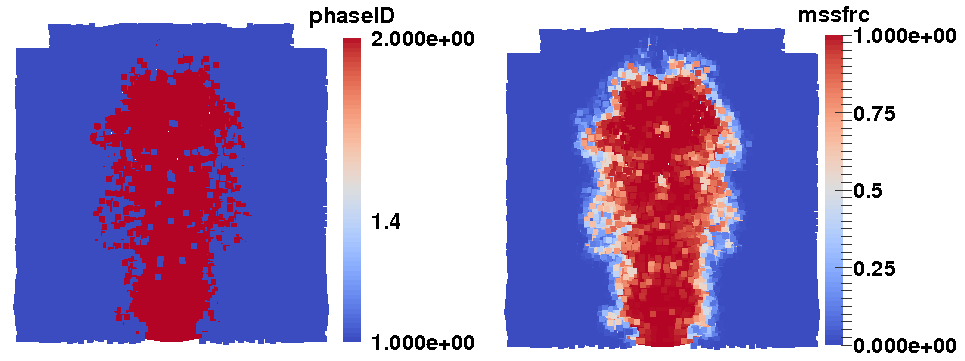
\includegraphics[width=12cm]{Interface.png}
\caption{In the left figure, the blue particles (phaseID=1) represent air particles the red ones (phaseID=2) represent erupted material. The right figure shows corresponding mass fraction. Mass fraction are evaluated based on Eq. (\ref{eq:gov-sph-d1}) and Eq. (\ref{eq:gov-sph-d1}) without any interface track or capture method.}
\label{fig:SPH-multiple-density}
\end{figure}
\subsection{Turbulence modeling with SPH}
Typically, turbulence fluctuations in a volcanic column occur on very different length scales, ranging from millimeters up to hundreds of meters. The entrainment of air and heat transfer are dominated by such turbulent fluctuations as turbulent exchange coefficient would be several magnitudes larger than molecular viscosity (and heat conduction) coefficient. One way to include enough turbulence in the model is to use SPH-SPS (SPH sub-particle-scale) method.
%\citep {gotoh2004sph, shao2006sph}. 
Another way is to use extremely fine resolution (The direct numerical simulation method) at the expense of much higher computational cost that results from both increase in number of particles and decrease in time steps constrained by CFL condition. Here we choose the SPH-SPS method to capture  momentum and energy exchange caused by smaller scale turbulence.\\
Even though free surface flow are in nature turbulent, detailed research in turbulence using the SPH method is rather scarce. Among the first papers on turbulence are the implementations of the $\alpha$ turbulence model \citep{holm1999fluctuation} by Monaghan \citep{monaghan2002sph} and the Reynolds averaged Navier-Stokes (RANS) approach by Violeau and Issa \citep{violeau2007numerical}. A first wall-bounded large eddy simulation (LES) was performed by Issa \citep{issa2005numerical}. An improved version of $SPH-\alpha$ method is proposed in 2011 by Monaghan \citep{monaghan2011turbulence}, which we refer to as $SPH-\varepsilon$ method. We will adopt $SPH-\varepsilon$ method in simulation of volcano plume. As most of these papers constrain their focus on incompressible or weakly compressible fluid. To simulate turbulence in plume, we need to extend existing incompressible turbulent modeling methods to compressible flows.\\
$SPH-\alpha$ model \citep{monaghan2002sph} is a powerful extension of the XSPH algorithm which reduces disorder at short length scales and retains the constants of the motion. But in that paper \citep{monaghan2002sph}, energy conservation equation is discretized in a way that is exactly the same as usual SPH. There is no special treatment on energy conservation equation. And the recent improved version \citep{monaghan2011turbulence} of $SPH-\alpha$ method focus on incompressible flow only. Actually, there are several additional terms in the averaged compressible Navier-Stokes equations besides the Reynolds stress term \citep{NASACompressibleTurbulence}. The averaged momentum equation for compressible flow are in the same form as that for incompressible flow, all of other additional terms except for turbulent stress term are in the energy equation). However, most turbulence modeling focuses on the Reynolds stress terms which are either solved directly or defined via a constitutive relation. Less attention is typically given to the other terms that need to be modeled. Most commonly, a Reynolds analogy is used to model the turbulent heat flux. Simulations of heat transfer or other scalar transfer in turbulent flow simply involve adding transport terms for thermal energy or species concentration, at the expense of greater storage and longer computing times but without other difficulties \citep{cebeci2013analysis}. We adopt this strategy in our simulation of turbulent heat transfer with $SPH-\varepsilon$. PDAC \citep{neri2003multiparticle} also adopted a Reynolds analogy in its turbulence modeling. The additional terms associated with molecular diffusion and turbulent transport in the energy equation are either modeled in different ways or neglected sometimes \citep{NASACompressibleTurbulence}. We neglect these terms in our simulation.\\
\subsubsection{$SPH-\varepsilon$ turbulence model}
In $SPH-\varepsilon$ method \citep{monaghan2011turbulence}, a turbulence model is constructed within the framework of SPH in such a way that general principles such as conservation of energy, momentum and circulation are satisfied using the ideas associated with the LANS (Lagrangian averaged Navier-Stokes equations). The basic idea of $SPH-\varepsilon$ is that determine a smoothed velocity $\widehat{\textbf{v}}$ by a linear operation on the unsmoothed velocity $\textbf{v}$. The SPH particles move with this smoothed velocity and the average motion of the fluid is determined by Eq. (\ref{eq:gov-update-pos-turbulence}):
\begin{equation}
\dfrac{d \textbf{x}_a}{dt} = \widehat{\textbf{v}}_a \label{eq:gov-update-pos-turbulence}
\end{equation}
Lagrangian equations contain extra term which represents the stresses induced by the smoothing. Once the form of the smoothing is chosen these stresses are determined. 
%The overall effect is to produce a redistribution of energy without dissipation. 
The typical LANS model uses a smoothed velocity $\widehat{\textbf{v}}$ 
defined in terms of the unsmoothed velocity $\textbf{v}$ by:
\begin{equation}
\widehat{\textbf{v}}(\textbf{x})=\int \textbf{v}(\textbf{x} \prime)G(\vert \textbf{x} \prime - \textbf{x} \vert, l) d\textbf{x} \prime
\end{equation}
Where $G$ satisfies:
\begin{equation}
\int G(\vert \textbf{x} \prime - \textbf{x} \vert, l) d\textbf{x} \prime =1
\end{equation}
and is a member of a sequence of functions which tends to the $\delta$ function in the limit where $ l\rightarrow 0$. A typical example is Gaussian.
The length scale $l$ determines the characteristic width of the kernel and the distance over which the velocity is smoothed.\\
It is common practice in $LANS-\alpha$ to use a differential equation for the smoothing rather than the integral form and finally reach to system of equations that need to be solved implicitly. In $SPH-\varepsilon$ method, a XSPH smoothing is adopted which will conserve linear and angular momentum. In this way solving of system of equations is avoided and it also makes the method simple to implement and cheap for computation. 
The discretized form of momentum equation is obtained through lengthy derivation based on Lagrangian equations. Derivation details and other discussions, such as conservation of momentum and energy, satisfactory of circulation theory, energy/momentum spectrum analysis based on Founrier transfer are detailed in Monaghan's paper \citep{monaghan2011turbulence}. Here we just have a brief summary on key steps.\\
The smooth that Monaghan adopted is:
\begin{equation}
\widehat{\textbf{v}}(\textbf{x})=\textbf{v}(\textbf{x})+ \epsilon \int (\textbf{v}(\textbf{x} \prime)-\textbf{v}(\textbf{x}))G(\vert \textbf{x} \prime - \textbf{x} \vert, l) d\textbf{x} \prime
\end{equation}
As function $G$ has the same feature as kernel function $w$, SPH approximation of the integration will lead to:
\begin{equation} \label{eq:SPH-epsilon-filtering}
\widehat{\textbf{v}}(\textbf{x})=\textbf{v}(\textbf{x})+\epsilon \sum_b m_b \dfrac{(\textbf{v}_b -\textbf{v})}{\rho _b} G(\vert \textbf{x} _b - \textbf{x} \vert, l)
\end{equation}
By making the replacement:
\begin{equation}
\label{eq:replacement-in-turb-derive}
\dfrac{G(\vert \textbf{x} _b - \textbf{x} _a \vert, l_a)}{\rho _b} \rightarrow \dfrac{K_{ab}}{M}
\end{equation}
Where $K_{ab} = l^d G_{ab}$, $M = \rho_0 l^d$ in which $d$ is the dimension and $\rho_0$ is initial density. $SPH-\varepsilon$ turbulence model is obtained after lengthy derivation:
\begin{equation}
\label{eq:monaghan-mom-turb}
\dfrac{d \textbf{v}_a}{dt} = -\sum_b [m_b (\dfrac{p_b}{\rho_b^2} + \dfrac{p_a}{\rho_a^2}) \bigtriangledown_aw_{a b}(h_a)] + \sum_b m_b \dfrac{\varepsilon}{2} \dfrac{\textbf{v}_{ab} \cdot \textbf{v}_{ab}}{M} \bigtriangledown_a K_{ab}
\end{equation}
Instead of using Eq. (\ref{eq:monaghan-mom-turb}) which is from Monaghan's paper, we make inverse replacement of Eq. (\ref{eq:replacement-in-turb-derive}) and notice that if $l$ is uniform and keep constant: 
%Please notice that the above equation is slightly different from the original equation in Monaghan's paper (Eq. (2.17)). The original equation is based on the assumption that density is uniform initially. This assumption is not general and atmosphere density is stratified in our plume simulation. And the slight modification will not influence following derivation if $l$ is uniform and keep constant because:
\begin{equation}
\nabla K_{ab} = \nabla (l^d G_{ab}) = l^d \nabla G_{ab}
\end{equation}
So the discretized momentum equation with $SPH-\varepsilon$ turbulence model in our simulation will be:
\begin{equation}
\label{eq:SPH-mom-epsilon-turb}
\dfrac{d \textbf{v}_a}{dt} = -\sum_b [m_b (\dfrac{p_b}{\rho_b^2} + \dfrac{p_a}{\rho_a^2}) \bigtriangledown_aw_{a b}(h_a)] + \sum_b m_b \Phi_{ab}\bigtriangledown_aG_{ab}(l_a)
\end{equation}
where 
\begin{equation}
\Phi_{ab}=\dfrac{\varepsilon}{2} \dfrac{\textbf{v}_{ab} \cdot \textbf{v}_{ab}}{\rho_b} 
\end{equation}
and take $\varepsilon = 0.8$ as recommended by JJ Monaghan.
\subsubsection{Turbulence heat transfer}
We adopt Reynolds analogy to get heat transfer coefficient due to turbulence.
Prandtl number is defined as:
\begin{equation}
Pr=\dfrac{C_p \mu}{\kappa}
\end{equation}
Where, $\mu$ is dynamic viscosity, $\kappa$ is thermal conductivity. And $\mu$  can be written in term of absolute viscosity (kinematic viscosity) as:
\begin{align}
\mu=\rho \nu
\end{align}
Then
\begin{equation}
\kappa=\dfrac{C_p \mu}{Pr}
\end{equation}
Typical value of $Pr_t$ for air is 0.7 $\sim$ 0.9 . We take $Pr_t=0.85$ for gases as recommended by Kays, William M \citep{kays1994turbulent} from summarizing of experimental results. 
JJ Monaghan \citep{monaghan2005smoothed} summarized the simulation of viscosity and heat conduction in his review on SPH. We will refer to his summary in our following discussion. The additional term in discretized momentum equation, Eq. (\ref{eq:SPH-mom-epsilon-turb}), is the turbulent shear stress term. 
Recall that viscosity term can be discretized with SPH as shown in Eq. (\ref{eq:art-vis-original}). 
Comparing of this term to physical viscous term for compressible gas shows that it has both bulk viscosity and shear viscosity, where shear viscosity coefficient is \citep{monaghan2005smoothed}:\\
\begin{equation}
\nu_t = S \nu
\end{equation}
with
\begin{equation}
S= 
\begin{cases} 
      \dfrac{1}{6} & for  \quad d=3 \\
      \\
     \dfrac{5}{24}  & for  \quad d=2 
\end{cases}
\end{equation}
The turbulent viscosity coefficient can be inferred from that form if we can reformulate the "turbulence stress" term in a form which is similar to molecular shear viscous term.
Reformulate the "turbulence stress" term:
\begin{equation}
 \sum_b \dfrac{\varepsilon}{2} \dfrac{m_b}{\rho_b} \textbf{v}_{ab} \cdot \textbf{v}_{ab} \nabla_a G_{ab}(l_a)= \sum_b \dfrac{\varepsilon}{2S} m_b \dfrac{\textbf{v}_{ab}}{\rho_b} \dfrac{S \textbf{v}_{ab} \cdot \textbf{x}_{ab}}{x_{ab}^2} \dfrac{x_{ab}^2}{\textbf{x}_{ab}} \nabla_a G_{ab}(l_a) 
\end{equation}
Then the turbulent viscosity coefficient will be
\begin{equation}
\nu_t = \dfrac{\varepsilon}{2S} \dfrac{\textbf{v}_{ab} \cdot \textbf{x}_{ab}}{\rho_b}
\end{equation}
Please notice that turbulent viscosity term has opposite sigh with molecular viscosity term in discretized momentum equation and there is a minus sign in the expression of $\Pi_{ab}$, they will cancelled out.
However, the above equation is correct only for 1D situation. For 2D or 3D, it is not easy to get the explicit expression of viscosity. \\
We adopt an alternative way: obtaining a value for each pair of particles instead of persisting on getting an analytical expression. Choosing smoothing function as the same as SPH kernel and the smoothing scale $l$ as the same as smoothing length $h$, the ratio between turbulent shear stress and physical shear stress is: 
\begin{equation}
\begin{split}
\Upsilon_{ab} &= \dfrac{\dfrac{\varepsilon}{2} \dfrac{\textbf{v}_{ab} \cdot \textbf{v}_{ab}}{\rho_b}}{\dfrac{S \nu}{\rho_{ab}} \frac{\textbf{v}_{ab} \cdot \textbf{x}_{ab}}{x_{ab}^2 + \eta^2 h_{ab}^2}} \\
 & = \dfrac{\varepsilon (x_{ab}^2 + \eta^2 h_{ab}^2)}{2 S \nu} \dfrac{\textbf{v}_{ab} \cdot \textbf{v}_{ab}}{\textbf{v}_{ab} \cdot \textbf{x}_{ab}}
\end{split}
\end{equation}
$\Upsilon_{ab}$ is essentially equivalent to ratio between turbulent viscous effect attributed by particle b on particle a and molecular viscous effect attributed by particle b on particle a. Turbulent viscosity can be easily obtained by:
\begin{equation}
\begin{split}
\nu_{t,ab} &= \nu \Upsilon_{ab} \\
&= \dfrac{\varepsilon (x_{ab}^2 + \eta^2 h_{ab}^2)}{2 S} \dfrac{\textbf{v}_{ab} \cdot \textbf{v}_{ab}}{\textbf{v}_{ab} \cdot \textbf{x}_{ab}}
\end{split}
\end{equation}
The corresponding turbulent thermal conductivity should be
\begin{equation}
\kappa_{t,ab}=\dfrac{\varepsilon \overline{C_{p,ab}} \overline{\rho_{ab}} (x_{ab}^2 + \eta^2 h_{ab}^2) \textbf{v}_{ab} \cdot \textbf{v}_{ab}}{2 S Pr_t\textbf{v}_{ab} \cdot \textbf{x}_{ab}}
\end{equation}
The term that used to prevent singularity now can be removed. 
\begin{equation}
\kappa_{t,ab}=\dfrac{\varepsilon \overline{C_{p,ab}} \overline{\rho_{ab}} x_{ab}^2 \textbf{v}_{ab} \cdot \textbf{v}_{ab}}{2 S Pr_t\textbf{v}_{ab} \cdot \textbf{x}_{ab} }
\end{equation}
We also need to prevent singularity, so: 
\begin{equation}
\kappa_{t,ab}= 
\begin{cases} 
      0 & if  \quad \textbf{v}_{ab}=0 \quad or \quad \textbf{x}_{ab}=0 \\
      \dfrac{\varepsilon \overline{C_{p,ab}} \overline{\rho_{ab}} x_{ab}^2 \textbf{v}_{ab} \cdot \textbf{v}_{ab}}{2 S Pr_t\textbf{v}_{ab} \cdot \textbf{x}_{ab} } & \text{otherwise}
\end{cases}
\label{eq:SPH-LANS-heat-conductivity}
\end{equation}
The heat conduction equation without source term is:
\begin{equation}
C_p \dfrac{dT}{dt} = \dfrac{1}{\rho} \nabla (\kappa \nabla T)
\end{equation}
Second spatial derivative can be approximated with SPH by following JJ Monaghan \citep{monaghan2005smoothed}. 
\begin{equation}
C_p \dfrac{dT}{dt} = \sum_b \dfrac{m_b}{\rho_a \rho_b} (\kappa_a + \kappa_b) (T_a - T_b) F_{ab} (h_a)
\end{equation}
Where
\begin{equation}
F_{ab} \textbf{x}_{ab} = \nabla _a w_{ab}
\end{equation}
And  $F_{ab} \leq 0$, which guarantees that heat flux will flow from hot to cold.
%JJ Monaghan \citep{cleary1999conduction} showed a simple alteration to the standard SPH formulation and ensures continuity of heat flux across discontinuities in material properties. 
Plug the turbulent thermal conductivity into the heat conduction equation:
\begin{equation}
\begin{split}
C_p \dfrac{dT}{dt} 
& = \sum_b \dfrac{m_b}{\rho_a \rho_b} (\kappa_a + \kappa_b) (T_a - T_b) F_{ab} (h_a) \\
 &= 2 \sum_b \dfrac{m_b}{\rho_a \rho_b} \dfrac{\overline{C_{p,ab}} \overline{\rho_{ab}} \varepsilon x_{ab}^2 \textbf{v}_{ab} \cdot \textbf{v}_{ab}}{2 Pr_t  S \textbf{v}_{ab} \cdot \textbf{x}_{ab} } (T_a - T_b) F_{ab} (h_a)
\end{split}
\end{equation}
Notice that the number 2 at the front of the equation comes from integration approximation of second order derivative \citep {cleary1999conduction}. By further simplification, we get:
\begin{equation}
C_p \dfrac{dT}{dt}
 =\dfrac{\varepsilon}{S  Pr_t}  \sum_b \dfrac{m_b}{\rho_a \rho_b} \dfrac{\overline{C_{p,ab}} \overline{\rho_{ab}} x_{ab}^2 \textbf{v}_{ab} \cdot \textbf{v}_{ab}}{\textbf{v}_{ab} \cdot \textbf{x}_{ab}} (T_a - T_b) F_{ab} (h_a)
\end{equation}
\subsubsection{Discretized governing Equation with $SPH-\varepsilon$ turbulence model}
Plug discretized turbulent stress term and turbulent heat transfer term into the momentum and energy equation, we got new discretized governing equation:
\begin{equation}
<\dfrac{d \textbf{v}_{\alpha}}{d t}>= 
-\sum_b [m_b (\dfrac{p_b}{\rho_b^2} + \dfrac{p_{\alpha}}{\rho_{\alpha}^2} + \Pi_{\alpha b} - \Phi_{\alpha b}) \bigtriangledown_{\alpha}w_{\alpha b}(h_{\alpha})]
-\sum_j [m_j (\dfrac{p_j}{\rho_j^2} + \dfrac{p_{\alpha}}{\rho_{\alpha}^2} + \Pi_{\alpha j} - \Phi_{\alpha j}) \bigtriangledown_{\alpha}w_{\alpha j}(h_{\alpha})]
+\textbf{g} \label{eq:gov-sph-v}
\end{equation}
With 
\begin{equation}
\Phi_{\alpha \beta}=\dfrac{\varepsilon}{2} \dfrac{\textbf{v}_{\alpha \beta} \cdot \textbf{v}_{\alpha \beta}} {\rho_{\beta}} 
\end{equation}
\begin{equation}
\begin{split}
<\dfrac{d e_{\alpha}}{d t}>
& = 0.5\sum_b [m_b \widehat{\textbf{v}_{\alpha b}} (\dfrac{p_b}{\rho_b^2} + \dfrac{p_{\alpha}}{\rho_{\alpha}^2} + \Pi_{\alpha b} - \Phi_{\alpha b}) \bigtriangledown_{\alpha}w_{\alpha b}(h_{\alpha})] 
 + 2 \sum_b \dfrac{m_b}{\rho_{\alpha} \rho_b} \kappa_{t,\alpha b} (T_{\alpha} - T_b) F_{\alpha b} (h_{\alpha}) \\
 & +0.5\sum_j [m_j \widehat{\textbf{v}_{\alpha b}}(\dfrac{p_j}{\rho_j^2} + \dfrac{p_{\alpha}}{\rho_{\alpha}^2} + \Pi_{\alpha j} - \Phi_{\alpha j}) \bigtriangledown_{\alpha}w_{\alpha j}(h_{\alpha})]
 + 2 \sum_j \dfrac{m_j}{\rho_{\alpha} \rho_j} \kappa_{t,\alpha j} (T_{\alpha} - T_j) F_{\alpha j} (h_{\alpha})
\end{split}
\label{eq:gov-sph-e}
\end{equation}
with $\kappa_{t,\alpha \beta}$ given by Eq. (\ref{eq:SPH-LANS-heat-conductivity}). 
As the particle-scale movement of flow is based on smoothed velocity, the velocity in the energy equation should also be smoothed.
The filtering process will be done according to Eq. (\ref{eq:SPH-epsilon-filtering}). Position of particles will be updated according to Eq. (\ref{eq:gov-update-pos-turbulence}). Smoothed velocity is also used while computing artificial viscosity $\Pi_{ab}$.\\
\subsection{Boundary conditions in SPH}
\subsubsection{Wall boundary condtion}
Traditionally either ghost particles that mirror SPH particles across the boundary \citep {ferrari2009new}, or boundary forces \citep {monaghan2009sph} have been used to impose the wall boundary conditions. One disadvantage of the later one is that the boundary forces tend to corrupt the solution in the neighborhood of such boundary forces. In addition, the natural way of imposing eruption boundary condition is using eruption ghost particles. To impose boundary conditions in a consistent way we adopt a modified version of ghost particle method \citep {kumar2013parallel} for wall boundary conditions. Stationary ghosts particles are deployed the same way as initial deployment of real particles. Instead of enforcing the symmetry particle by particle, symmetric field across the boundary is explicitly enforced. Ghost positions are reflected into the domain and physical properties are calculated at these reflected positions by SPH interpolations. It should be noted that ghost particles are not used for these interpolations. Assign all properties at the corresponding reflect position to that ghost particle except for velocity. We assign a velocity to each wall ghost particles that is the negative of the interpolated velocity of its corresponding reflection inside the fluid domain. By this way, the no-slip wall boundary condition (Eq. (\ref{eq:wall_bc_v})) is imposed naturally. These wall ghost particles will serve as neighbors in momentum and energy update. Implementation details about this method can be found in \citep {kumar2013parallel}. As these wall ghost particles keep stationary, there will be no mass flux on the boundary (Eq. (\ref{eq:wall_bc_rho}) and (\ref{eq:wall_bc_xi})). In addition, as temperature is also symmetric with respect to the boundary, the gradient of temperature will vanish on the wall boundary and hence no internal energy flux on the wall boundary (Eq. (\ref{eq:wall_bc_e})). 
\subsubsection{Eruption boundary condition}
The natural way of imposing eruption boundary condition is using ghost particles which moves with eruption velocity and bears the temperature of erupt material. A parabolic velocity profile which represents a fully developed Hagen-Poiseuille flow is used to determine the particle velocity. The detailed shape of the parabolic profile will determined based on averaged eruption velocity (Eq. \ref{eq:erupt_bc_v}). The correctness of eruption boundary condition for density (Eq. (\ref{eq:erupt_bc_rho})) can be guaranteed by choosing mass of erupted ghost particles given distribution of these particles. The internal energy associated with these particles are set to a value so that Eq. (\ref{eq:erupt_bc_e}) is satisfied. The mass fraction of erupted material (Eq. (\ref{eq:erupt_bc_xi})) is automatically satisfied as all particles in the eruption conduit are of phase 2. The density, momentum, and internal energy of these eruption ghost particles will not be updated before they move above ground. As soon as they enter the atmosphere, these ghost particle will be shift to real particles and their physics properties and position will be updated based on discretized governing equations. New ghost particle will be added at the bottom of the eruption conduit as these existing ghost particles move upwards.\\
\subsubsection{Pressure boundary condition}
An other boundary in this model is pressure outlet boundary. For flow in a straight channel, it is possible to treat the exit the same as the entry with a prescribed velocity profile. For flow with more complex channel, an exit far downstream of the flow disturbance is also feasible. However, the natural boundary condition (Eq.  (\ref{eq:pressure_bc_p})) is more suitable for plume simulation where the outlet is open atmosphere. The way we impose pressure boundary condition is simple: adding several layers of pressure ghost particles surrounding the real atmosphere particles. Physics properties except for velocity (pressure, density, temperature) are determined based on the elevation of particles. Velocity is set to zero for static atmosphere. The physics properties for pressure ghost particles will not be updated while these for real particles will be updated at every time step. As position of all pressure ghost particles are keep constant, we are essentially imposing a static pressure boundary condition. Real particles that moves out the pressure boundary will be removed.\\
As simulation progress, change in position and physical properties of real particles near pressure boundary boundaries might corrupt pressure boundary condition that was established initially. This shortcoming is relieved by choosing a larger computational domain so that boundaries that might be corrupted will locate far away from turbulent mixing area. In addition, to avoid enlarging fluctuation, we add another constrain on time step: 
\begin{equation}
\Delta t \leq CFL_p \dfrac{h}{v}
\end{equation}
Where $CFL_p$ is a safety coefficient which has similar function as the normal $CFL$ number. Too small $CFL_p$ will slow down simulation while too large $CFL_p$ will lose its ability of mitigate numerical fluctuation near the boundary. The proper $CFL_p$ is determined by series of simulation tests. \\
In subfigure b of Fig. \ref{fig:bc_and_domain_decomp}, different type of boundary conditons are marked with different color. The red portion are main computational domain. 
\begin{figure}
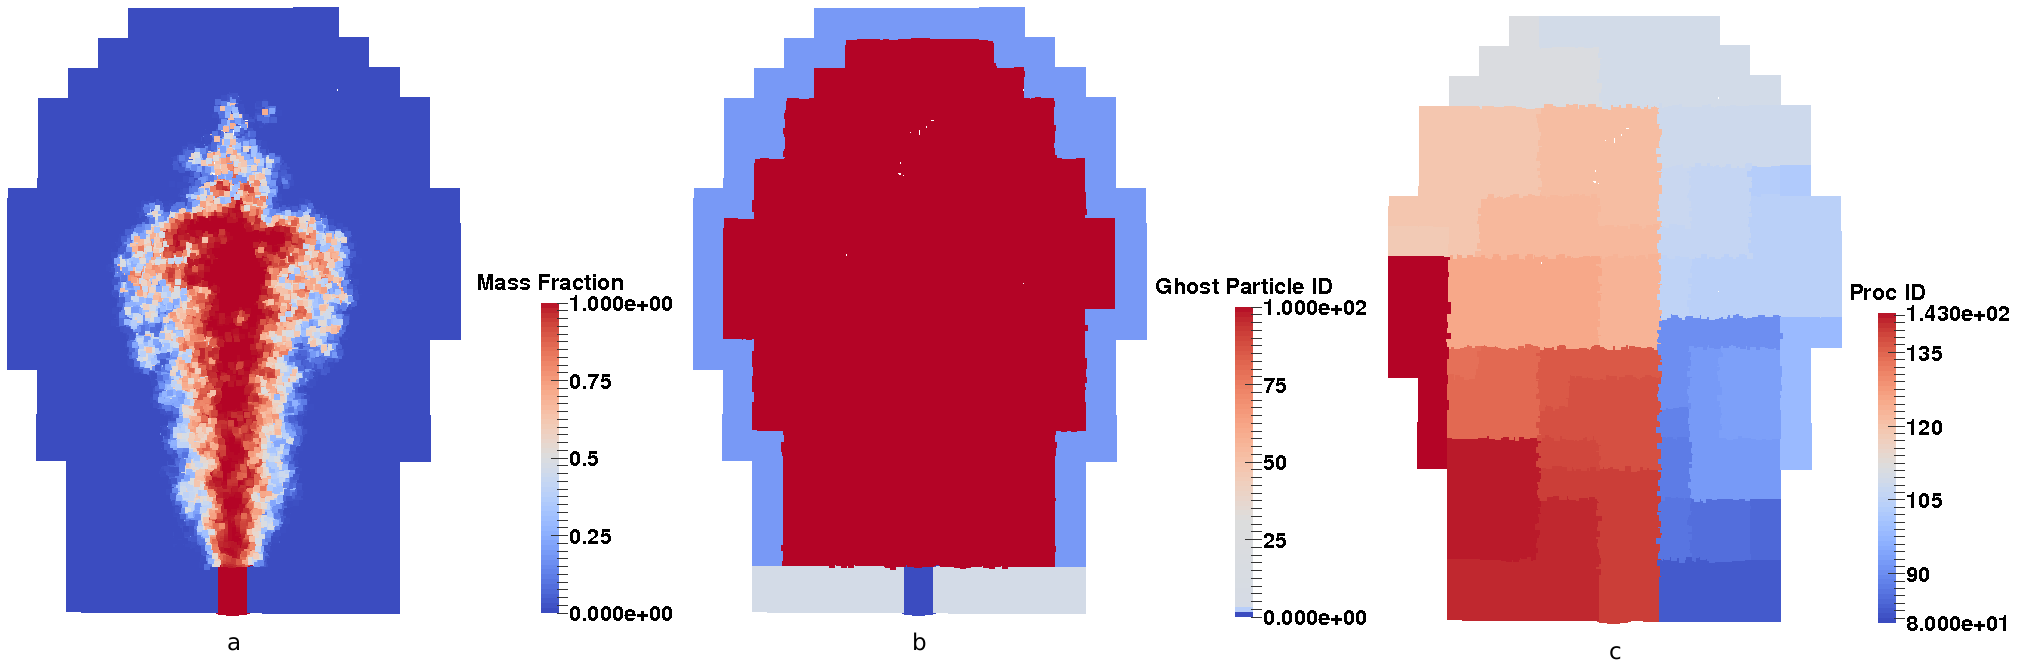
\includegraphics[width=18cm]{t120_bc_proc.png}
\caption{A cross section view of the simulation domain. Subfigure a shows the mass fraction of a plume simulation. Subfigure b shows all boundary conditions: the dark blue is for velocity inlet boundary, the light blue is for pressure outlet boundary, the gray is for no-slip wall boundary condition. Ghost particle ID of All real particles are set to 100, so is 100 in b. Subfigure c shows the cross section view of domain decomposition based on SFC. The simulation is conducted on 144 processors (12 nodes with 12 cores each node), so there are 144 subdomains in total.}
\label{fig:bc_and_domain_decomp}
\end{figure}
\subsection{Parallellism and performance}
One disadvantage of 3D model is that it usually takes much longer time than 1D models to complete one simulation. This disadvantage further preventing doing simulation with finer resolution and accounting for more physics in one model. Non-intrusive uncertainty analysis which is commonly adopted in hazard forecasting requires finishing multiple simulations within a given time window. High performance computing provides a powerful routine for relieving the misery. Among existing CPU parallel SPH schemes, most of them focus on neighbors searching algorithm and dynamic load balancing (eg. \citep {ferrari2009new, crespo2015dualsphysics}). Less attention has been paid to developing of more flexible data management schemes for more complicated problems. Motivated by techniques developed for mesh based methods, we develop a complete framework for parallelizing SPH program with MPI standard model allowing flexible and efficient data access in this paper.\\
Any implementation of SPH code requires efficient searching and updating of neighbors during simulation. Of the many choices possible for this we adopted a background grid which was proposed by Monaghan and Lattanzio \citep {monaghan1985refined} and is quite popular in parallel SPH. The background grid is also used for domain decomposition in SPH. We refer to the elements of background grid, namely squares for two dimensions and cubic for three dimension, as buckets. 
As for the actual storage of data representing the physical quantities associated to each particle, different strategies have been adopted in existing implementations of SPH.
In both SPHysics and DualSPHysics \citep {crespo2015dualsphysics}, the physical quantities of each particle (position, velocity, density...) are stored in arrays, and the particles (and the arrays with particle data) are reordered following the order of the cells. This has two advantages: 1) access pattern is more regular and more efficient, 2) it is ease to identify the particles that belong to a cell by using a range since the first particle of each cell is known. But adding, deleting and especially accessing of particles are cumbersome. Ferrari \citep {ferrari2009new} adopted linked lists using pointers so that particles can be deleted or added during the simulation. Storage problems caused by fix-size arrays are thereby also eliminated. We define C++ classes which contain all data of particles and buckets. As for the management of data, we adopt hash tables to store pointers to particles and buckets, which give us not only flexibility of deleting and adding elements, but also quicker access compared with linked list. Instead of using the "nature manner" to number particles, we adopt SFC based index to give each particle and background bucket an unique identifier -- a strategy known to preserve some locality at minimal cost. The SFC based numbering strategy is further extended to include time step information so that particles added at the same position but different time will have different identifiers. 
As for domain decomposition, even though more complicated graph-based partitioning tools \citep {biswas1999experiments} might get higher quality decomposition, they requires much more effort in programming and computation. So we adopt an easy-programming scheme based on SFC \citep {patra1999efficient}. Subfigure c of Fig. \ref{fig:bc_and_domain_decomp} shows a cross section view of domian decomposition.\\
We will provide a supplementary documentation describing details about the data structure, domain decomposition, load balancing and domain adjusting.
\begin{figure}[!t]
\centering
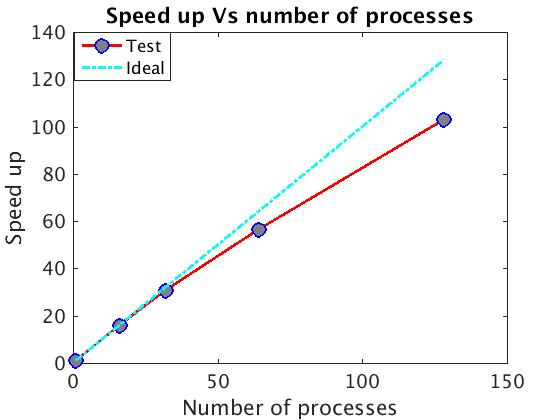
\includegraphics[scale=0.35]{strong}
\caption{Strong scalability test results}
\label{fig:strong_scale}
\end{figure}
\begin{figure}[!t]
\centering
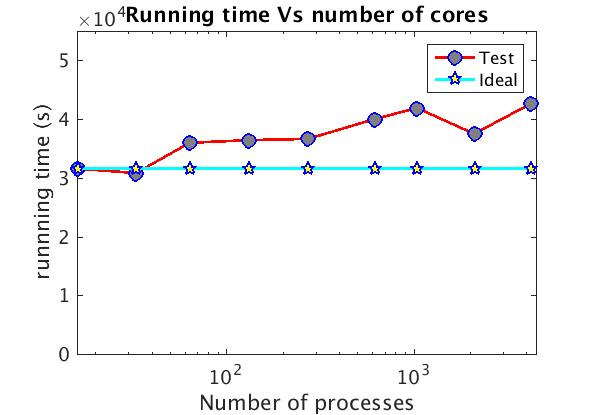
\includegraphics[scale=0.35]{weak_scale}
\caption{Weak scalability test results}
\label{fig:weak_scale}
\end{figure}
\begin{figure}[!t]
\centering
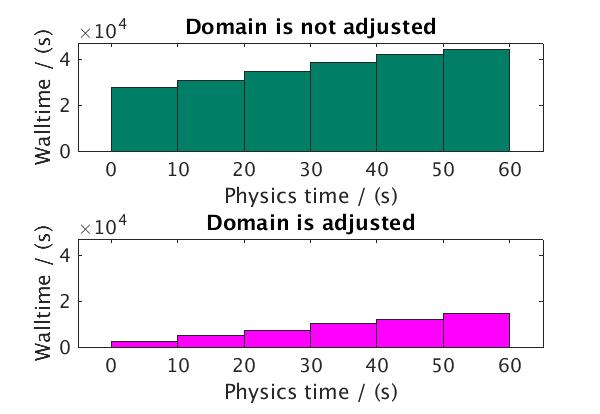
\includegraphics[scale=0.35]{adj_vs_no}
\caption{The effect of domain adjusting on simulation time. The figure on the top shows simulation time without domain adjusting, the figure on the bottom shows simulation time with domain adjusting. Different bins represent simulation time up to specific physics time indicated by $x$ axis.}
\label{fig:adj_vs_no}
\end{figure}
Experiments have been carried out on CCR (the computational cluster of Center for Computational Research) at Buffalo. E5645 CPUs running at 2.40GHz clock rate with 4GB memory per core on a Q-Logic Infiniband is used in these tests. Each node comprise of two sockets with 6 of these cores. Memory and level 3 cache are shared on each node. The initial domain is $[-4.8km,4.8km] \times [-4.8km,4.8km] \times [0km, 6km]$. Almost linear speed up is observed in our strong scalability test (Fig. \ref{fig:strong_scale}).
The weak scalability test is conducted with the same initial domain and various smoothing lengths. Each simulation is run for 400 steps. The average number of real particles of each process is kept constant at $25900$. As shown in Fig. \ref{fig:weak_scale}, simulation times increase around $1/3$ when number of cores increase from 16 to 4208. For the test problem in this section, the volcanic plume will finally reach to a region of $[-30km \,\,\, 30km] \times [-30km\,\,\,30km] \times [1.5km\,\,\,40km]$ after around 400 seconds of eruption. When numerical simulation goes up to 90 seconds, the plume is still within a region of $[-10km\,\,\,10km] \times [-10km\,\,\,10km] \times [0km\,\,\,25km]$. This implies that adjusting of domain can avoid computing large number of uninfluenced air particles, especially for the beginning stage of simulation. A domain adjusting algorithm is designed and implemented in our code. Figure \ref{fig:adj_vs_no} shows that simulation time of the test problem is greatly reduced when we adopt the domain adjusting strategy in our code.
\section{Verification and validation} \label{sec:verification-validation}
We will now present a series of numerical simulations to verify and validate the model. Plume-SPH is first verified by a JPUE simulation. Velocity and mass fraction distribution both along the central axis and cross transverse are compared with experimental results. The pattern of ambient particles entrainment is also clearly shown. Then a simulation of representative strong volcano plume is conducted. Both global variables and local variable are comparable with simulation results from existing 3D plume models. Analysis on evolution of plume shows detailed air entrainment mechanism. 
\subsection{Simulation of JPUE}
JPUE can be considered as a simplified volcanic plume. While the effect of stratified atmosphere and the effect of expansion due to high temperature in volcanic plume are not represented, JPUE reproduces the entrainment due to turbulent mixing which is one of the key elements in volcanic plume development. There exist consistently good experimental data \citep { list1982turbulent,dimotakis1983structure, papanicolaou1988investigations} that describe the JPUE flow field giving an insight into details of JPUE, such as transverse velocity and concentration profile. In this section, we will verify that our code and the $SPH-\varepsilon$ turbulence model is able to reproduce feature of turbulent entrainment by a JPUE simulation.\\
As many of these experiments were conducted with liquid, we replace the original equation of state (Eq. (\ref{eq:EOS})) with a weakly compressible Tait equation of state \citep {becker2007weakly} (see Eq. (\ref{eq:EOS-Tait})) to avoid solving the Poisson equation.
\begin{equation}
p=B[(\dfrac{\rho}{\rho_0})^{\gamma}-1]
\label{eq:EOS-Tait}
\end{equation}
with $\gamma=7$ and $B$ is evaluated by:
\begin{equation}
B=\dfrac{\rho_0 c^2}{\gamma}
\end{equation}
Where $c$ is speed of sound in the liquid. Energy equation is actually decoupled from momentum and mass conservation equation by using this EOS. In addition, the "atmosphere" is assumed to be uniform and gravity is set to be zero. We set the temperature and density of ejected material from the vent the same as its surrounding ambient. This will further simplify the scenario for the convenience of studying turbulent mixing. One overall feature of JPUE is "self-similarity" which means that the evolution of the JPUE is determined solely by the local scale of length and velocity which theoretically account for the fact that the rate of entrainment at the edge of JPUE is proportional to a characteristic velocity at each height. As a results, physical and numerical experiments do not necessary to have exactly the same setups and are compared on a non-dimensional basis.\\
\begin{figure}
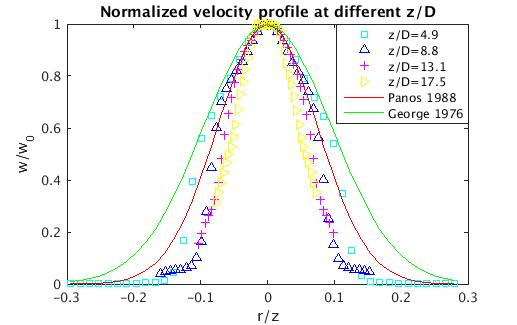
\includegraphics[width=8cm]{vel_cross}
\caption{Dimensionless velocity distribution across the cross-section.}
\label{fig:JPUE_cross-section_vel}
\end{figure}
\begin{figure}
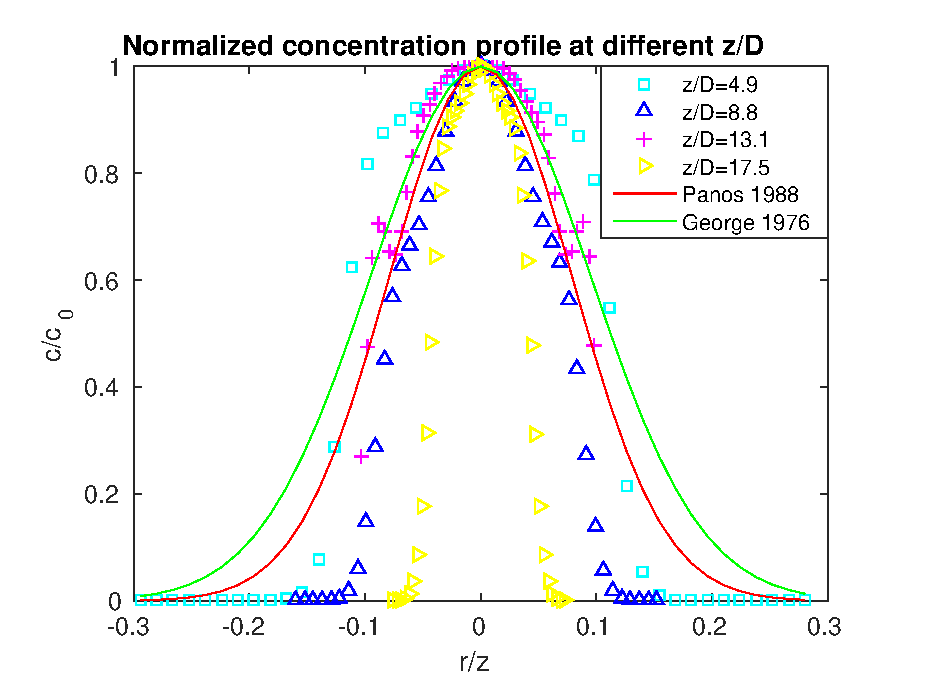
\includegraphics[width=8cm]{conc_cross}
\caption{Dimensionless concentration distribution across the cross-section.}
\label{fig:JPUE_cross-section_conc}
\end{figure}
\begin{figure}
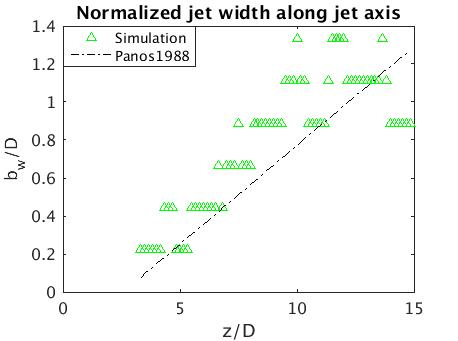
\includegraphics[width=8cm]{velo_along_axis}
\caption{Dimensionless velocity distribution along centraline.}
\label{fig:JPUE_along-axis_vel}
\end{figure}
\begin{figure}
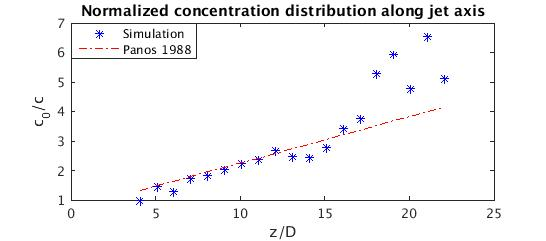
\includegraphics[width=8cm]{conc_along_axis}
\caption{Dimensionless concetration distribution along centraline.}
\label{fig:JPUE_along-axis_conc}
\end{figure}
A three dimensional axisymmetric JPUE which ejects from a round vent is simulated and results are compared with experiments \citep {george1977turbulence, papanicolaou1988investigations} for verification purpose. Experimental data of concentration and velocity distribution across the cross-section was fit into a Gaussian profile: $\dfrac{\varphi}{\varphi_c}=exp[-coef (\dfrac{r}{z})^2)]$ (solid line) even though there is no priori reason. Panos \citep{papanicolaou1988investigations} also fit concentration distribution and jet width based on velocity along central line into a straight line : $\dfrac{\varphi_0}{\varphi_c}=slope (\dfrac{z}{D} + intercept)$ (dash line). Where $\varphi$ is either velocity or concentration, the subscript $c$ represents the centreline, subscript $0$ represents the cross-sectionally averaged exit value. $r$ is the distance from the centreline on any cross-section. $z$ is the axial distance from the origin of the jet transverse section under consideration. $D$ is the diameter of vent. 
The coefficient $coef$ for concentration is 80 and 50 respectively according to Panos and George. $coef$ for velocity is 90 and 55 respectively according to Panos and George. 
$slope$ for jet width based on velocity is 0.104 and for concentration is 0.157. $intercept$ for jet width based on velocity is 2.58 while that for the concentration is 4.35.\\
Although both velocity and concentration are found to be well matched with experimental results, a small disparity in both velocity and concentration are observed near the boundary of the jet. There are several factors that would attribute to such disparity. Reynolds number is not reported in many experiments assuming a high enough Reynolds number. In addition, some details of the experiments, such as exit velocity profile, viscosity of the experimental liquid, are not reported, neither. These factors prevent us from numerically reproducing these experiments in an exact way as they were conducted. However, the features of JPUE is correctly reproduced with our code.\\
We also investigated the mixing due to turbulence in JPUE simulation by checking the mixture of two phases. It is shown in Fig. \ref{fig:Turb_mixing} that the ejected material and ambient fluids are mixed through eddies at the outer shear region. And the inner dense core dispersed gradually due to erosion of the outer shear region. Hence, our confidence in the numerical correctness of our code  is greatly reinforced.
%What need to be noticed is that the mass of particle of phase 1 (blue) is 8 time of that of phase 2 (red). It is a trade off between resolution and computational expense to give particle of two phases different particles mass. Both advanced SPH techniques like adaptive particles size and better data management and access strategies need to be exploited to address this issue.
\begin{figure}
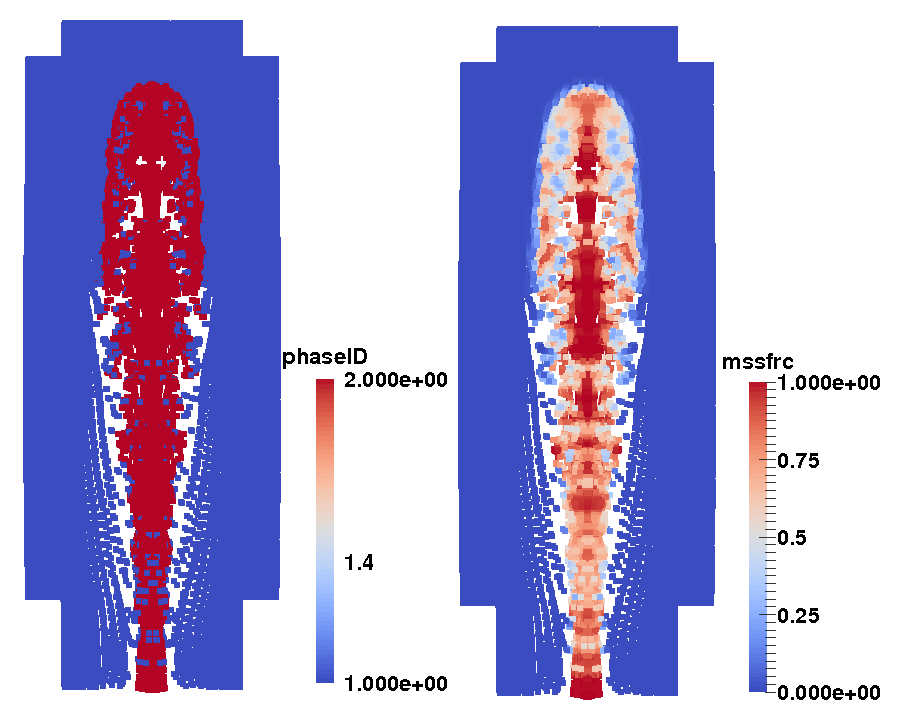
\includegraphics[width=8cm]{JPUE_entrainment.png}
\caption{Left figure shows particle distribution. The right figure shows the mass fraction of erupted material at the moment corresponding to left figure. Particles of phase 1 (blue) are gradually entrained and mixed with erupted particles (red) as jet flows down stream. What need to be noticed is that the mass of particle of phase 1 (blue) is 8 time of that of phase 2 (red). It is a trade off between resolution and computational expense to give particle of two phases different particles mass.}
\label{fig:Turb_mixing}
\end{figure}
\subsection{Simulation on Plume}
The development of volcano plume is more complicated than JPUE in several aspects. Besides turbulent entrainment of ambient fluids, development of volcano plume also involves heating up of entrained air and expanding in a stratified atmosphere. A strong eruption column without wind is tested in this section for the purpose of further verification and validation. Input parameters, material properties and atmosphere are chosen to be the same as the strong plume no wind case in an inter-comparison study on eruptive column models \citep{costa2016results}. The strong plume scenario was based on climactic phase of the Pinatubo eruption (Philippines, 15 June 1991). Material properties are selected based on properties of Pinatubo and Shinmoe-dake eruption. Both global variable and local variables are compared with existing models. Then plume evolution process is investigated.  
\subsubsection{Global and local variables}
One of the key global quantities of great interest is the altitude to which the plume rises. The top height predicted by our model is around 40 km which agrees well with other plume models. For example, the height predicted by PDAC is 42500 m, by SK-3D is 39920 m, by ATHAM is 33392 m, by AHSEE is 36700 m. As for local variables, the profiles of integrated temperature, density, mass fraction of entrained air, gas mass fraction, mass fraction of solid and the radius of the plume as a function of height are compared with existing 1D and 3D models in Fig. \ref{fig:strong_local_temp} ~ \ref{fig:strong_local_radius}. To get rid of significant fluctuations in time and space we did time averaging and spatial integration of the dynamic 3D flow fields by following Cerminara \citep {cerminara2016large}.
As particles distribute in the space in a disordered manner. We first project simulation results (on disordered particles) onto a pre-defined grid before doing time average and spatial integration. The interpolation method is the basic SPH kernel based interpolation.
\\
\begin{figure}
\center
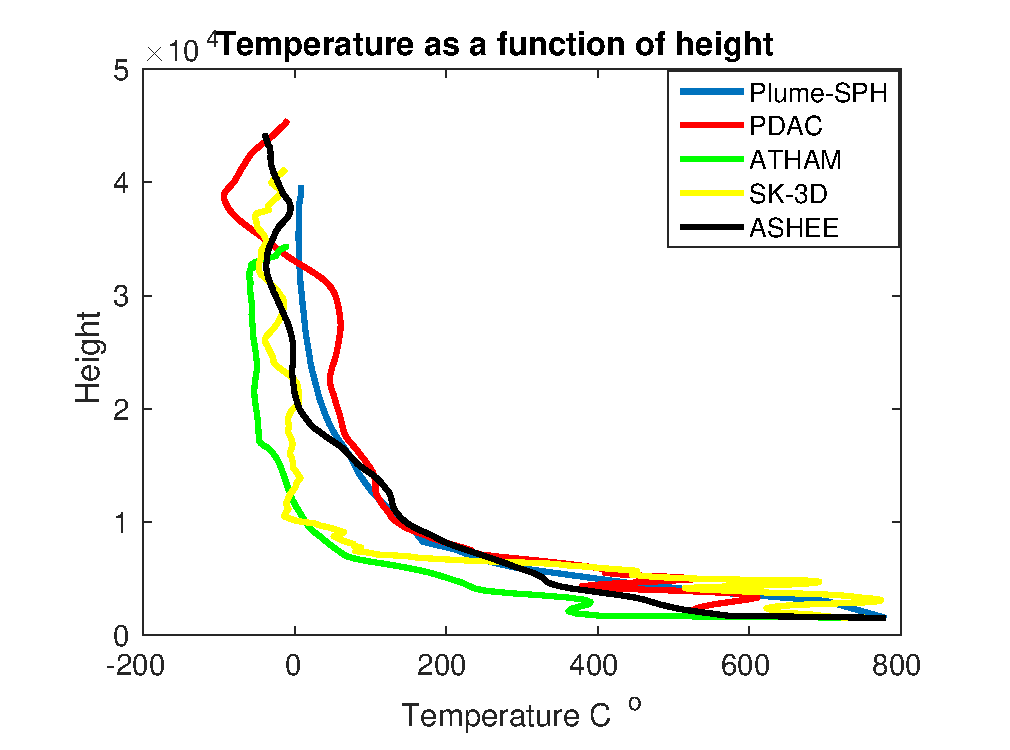
\includegraphics[width=5cm]{Temp}
\caption{Temperature as a function of height}
\label{fig:strong_local_temp}
\end{figure}
\begin{figure}
\center
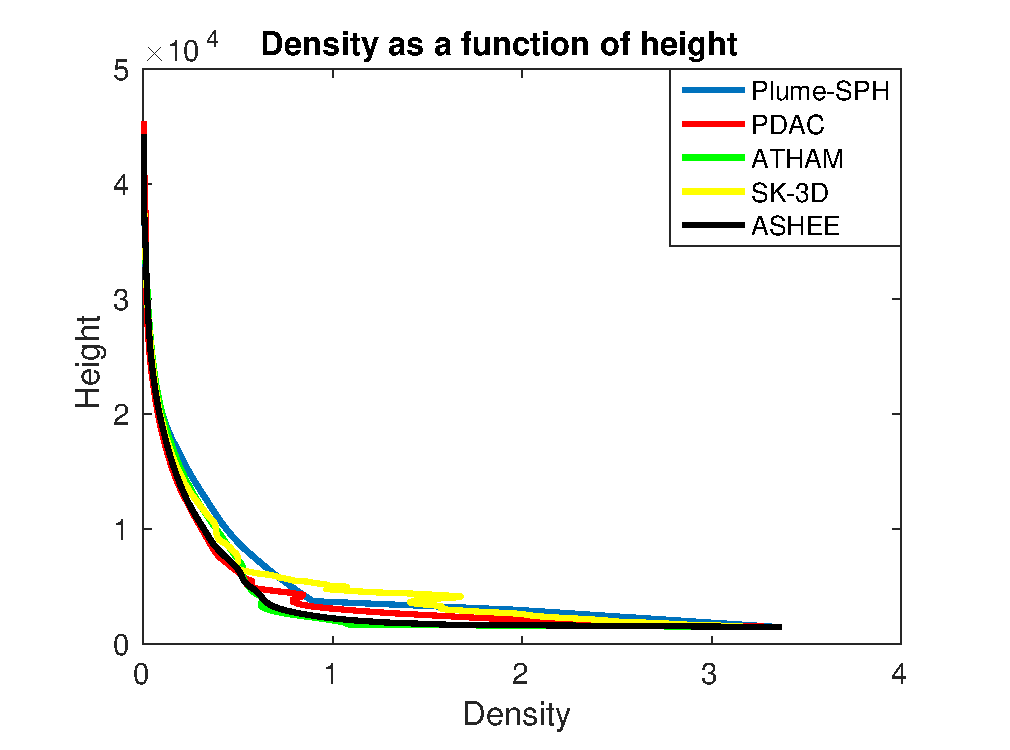
\includegraphics[width=5cm]{density_strong}
\caption{Density of the strong plume without wind after reaching its top height}
\label{fig:strong_local_density}
\end{figure}
%\begin{figure}
%\center
%\includegraphics[width=5cm]{velocity_strong}
%\caption{Velocity of the strong plume without wind after reaching its top height}
%\label{fig:strong_local_velocity}
%\end{figure}
The profiles of local variables match well with simulation results of existing 3D models in general sense. The basic phenomena in volcano plume development is correctly captured by our model.
%: the plume first rises up to its top height and then falls down to the neutral buoyancy height and starts expanding.\\
%
\begin{figure}
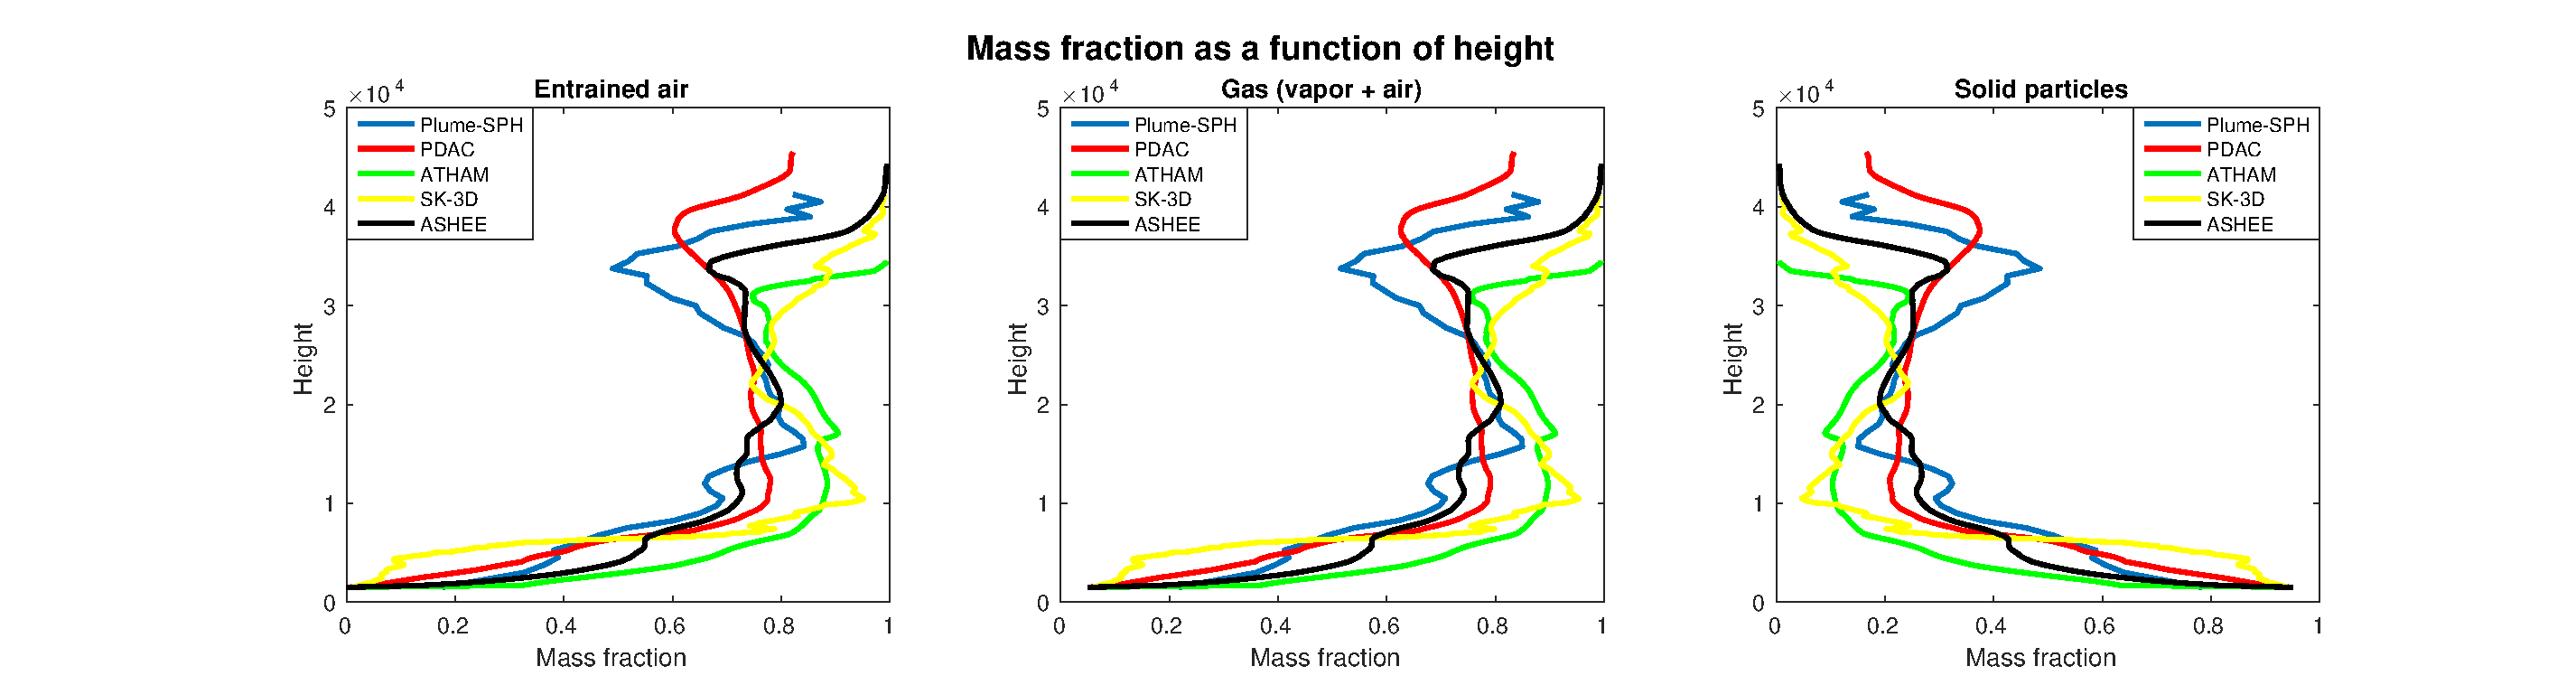
\includegraphics[width=15cm]{msfrac}
\caption{The mass fraction of entrained air, gas, and solid as a function of height.}
\label{fig:strong_plume_mass_fraction}
\end{figure}
%
As the height increase, the amount of entrained air will increase. Around the neutral height, where the umbrella expanding, the entrainment of air shows a slight decrease due to lack of air surrounding the column at that height. The profile for gas, which account for both air and vapor, shows a very similar tendency as that of entrained air. First of all, vapor condense is not considered in our model. In addition, as we assume that erupted material behaves like a single phase water, the mass fraction of gas will simply be a function of entrained air (Eq. (\ref{eq:gas-frac-express})). Among these 3D models, ATHAM takes vapor condense into account and Eq. (\ref{eq:gas-frac-express}) does not hold for ATHAM. However, the profile of entrained air and profile of gas predicted by ATHAM are still very close to each other which implies that ignoring of water phase change is a valid assumption for eruptions similar to this test case (strong plume with erupted water fraction in erupted material less than 5\%). Because air occupies a larger portion of the gas and plays a more significant role. As for mass fraction of solid, similarly, we have Eq. (\ref{eq:solid-frac-express1}) or Eq. (\ref{eq:solid-frac-express2}). PDAC which treat particles of two different sizes as two separate phases got similar mass fraction profile. Which implies that our model is at least valid for eruptions similar to the test case. 
\begin{equation}
n_a + n_g = n_a + (1-n_a) n_{g0}
\label{eq:gas-frac-express}
\end{equation}
\begin{equation}
n_s = (1 - n_a) (1- n_{g0})
\label{eq:solid-frac-express1}
\end{equation}
\begin{equation}
n_s = 1 - (n_a + n_g)
\label{eq:solid-frac-express2}
\end{equation}
%
\begin{figure}
\center
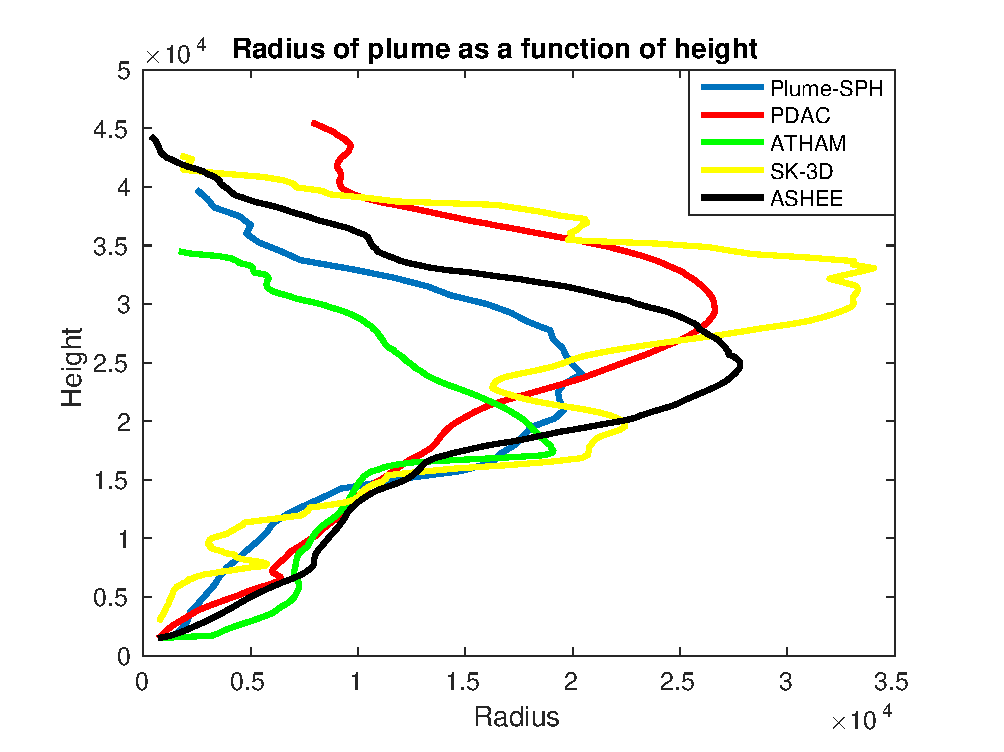
\includegraphics[width=5cm]{radius_strong}
\caption{Radius of the strong plume without wind after reaching its top height}
\label{fig:strong_local_radius}
\end{figure}
%
With more cool air entrained into the plume and mixing with hot erupted material, the temperature of the plume decreases as the height increase as shown in Fig. \ref{fig:strong_local_temp}. In the meanwhile, bulk density decrease due to entrainment and expansion (Fig. \ref{fig:strong_local_density}).\\
Our model adopts the same assumptions and governing equations as SK-3D. However, there is still a big disparity between the profiles of local variables of our model and 3K-3D. One of the big differences between our model and 3K-3D is that we adopt a LANS type of turbulence model while 3K-3D adopts a LES (large eddy simulation) turbulence model. This implies that turbulence model plays a critical role in plume simulation.
\subsubsection{Evolution of plume} 
\begin{figure}
\center
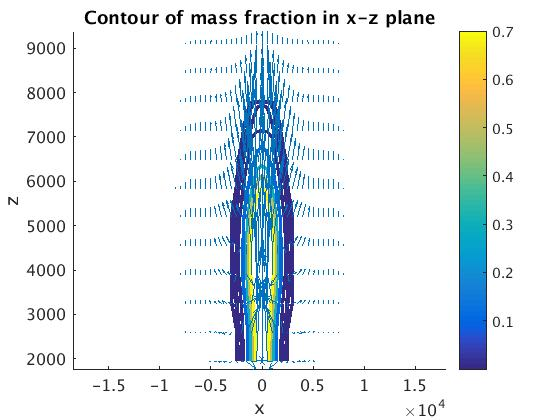
\includegraphics[width=5cm]{t15}
\caption{Contour of mass fraction and velocity quiver at 15 seconds, column rises up quickly due to initial momentum.}
\label{fig:strong_t15}
\end{figure}
\begin{figure}
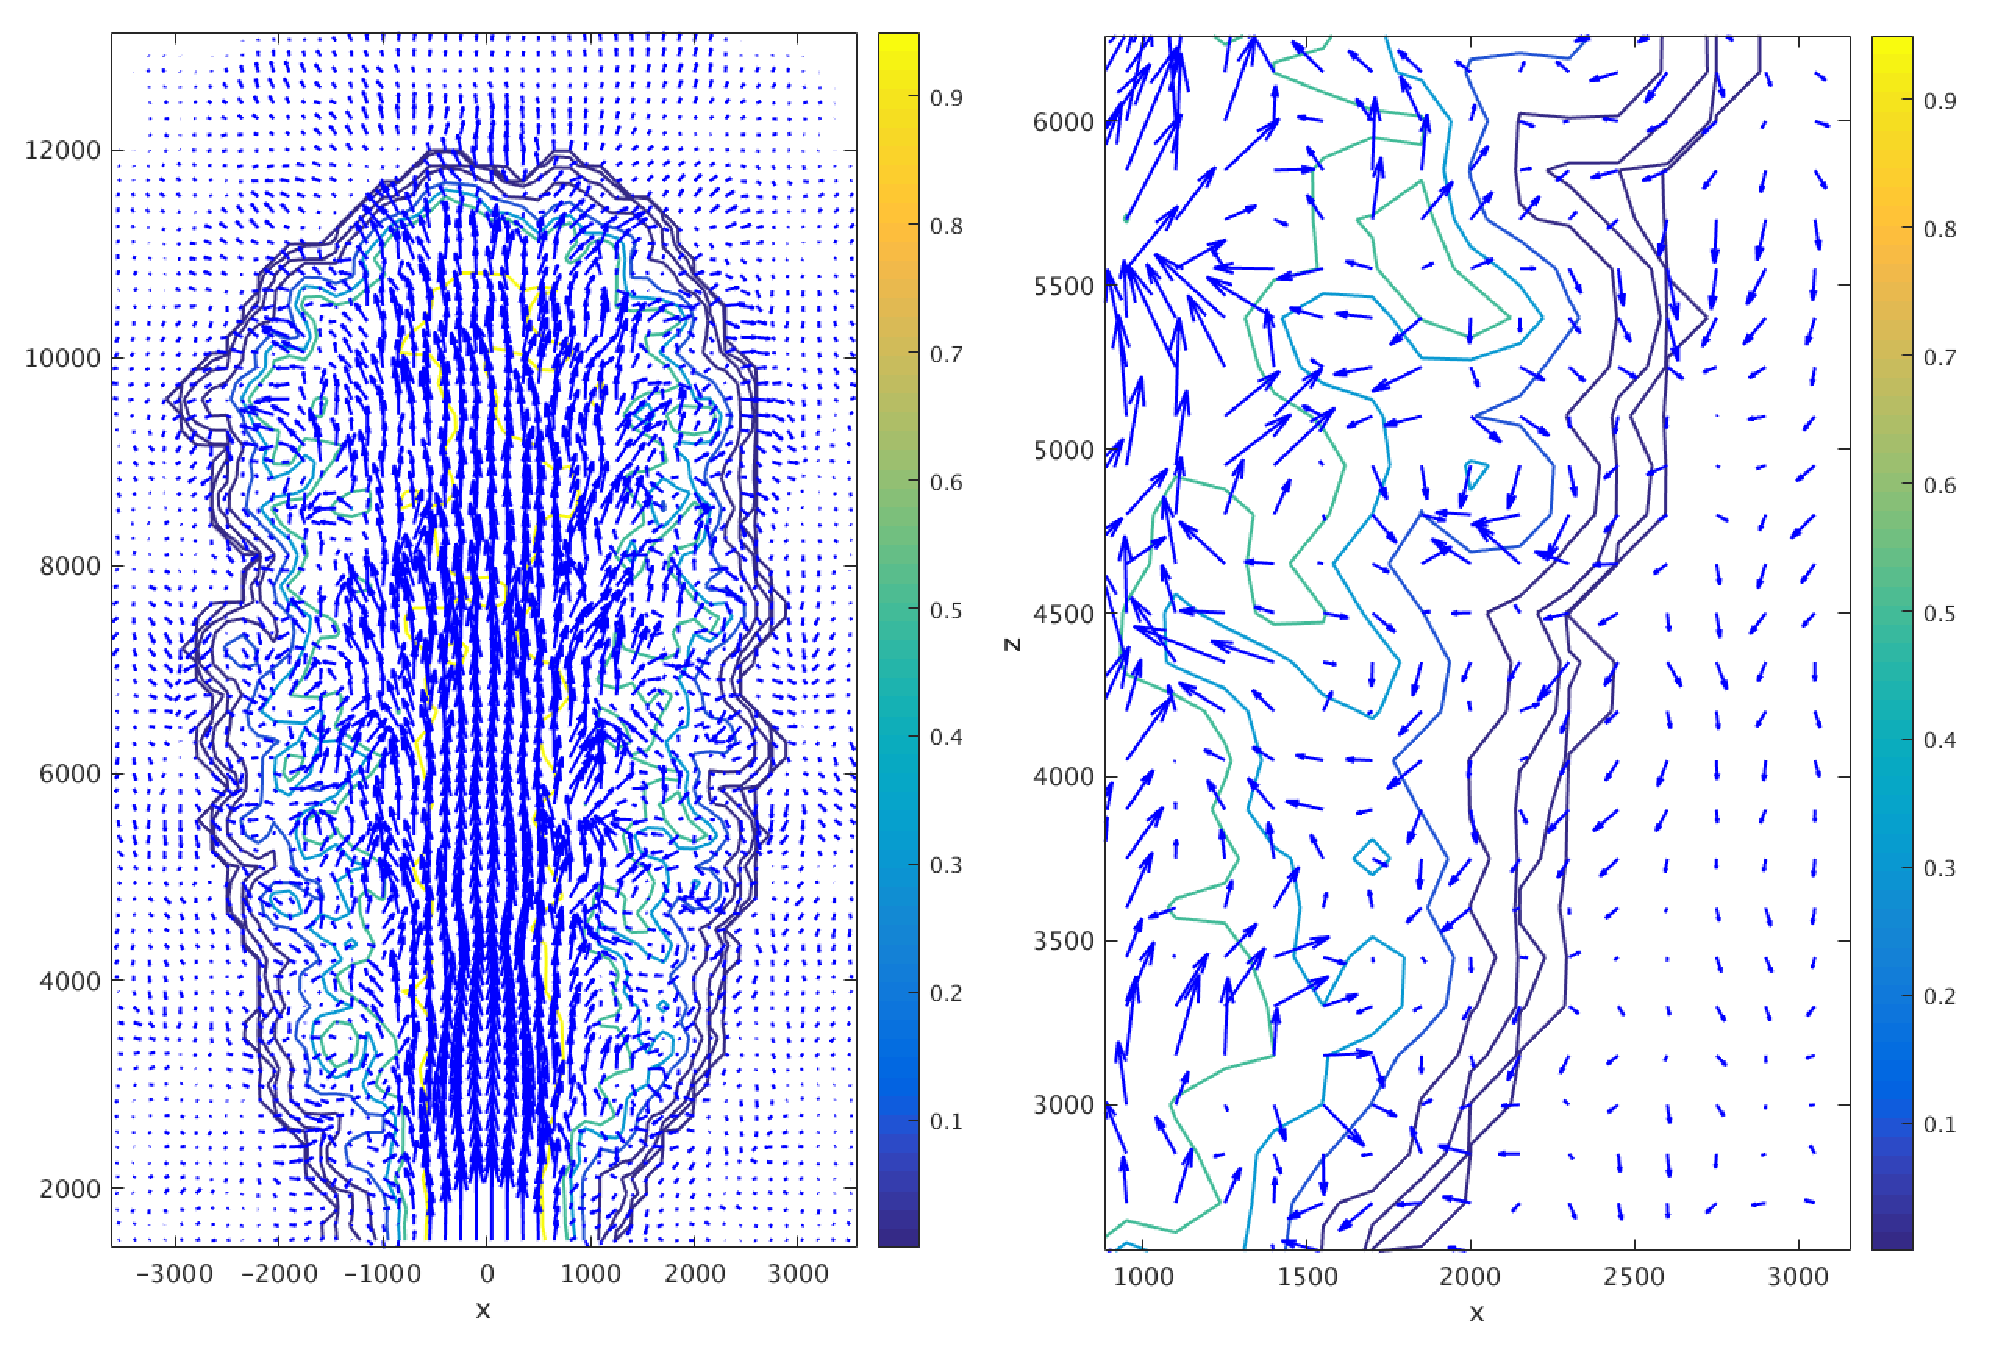
\includegraphics[width=10cm]{t50}
\caption{Contour of mass fraction and velocity quiver at 50 seconds, column keeps rising up and at the same time entraining air into the plume at the outer shear region. The entrainment of air is shown in a zoomed view in which the velocity quiver clearly shows entrainment of air into the plume at the margin of plume.}
\label{fig:strong_plume_t50}
\end{figure}
\begin{figure}
\center
{
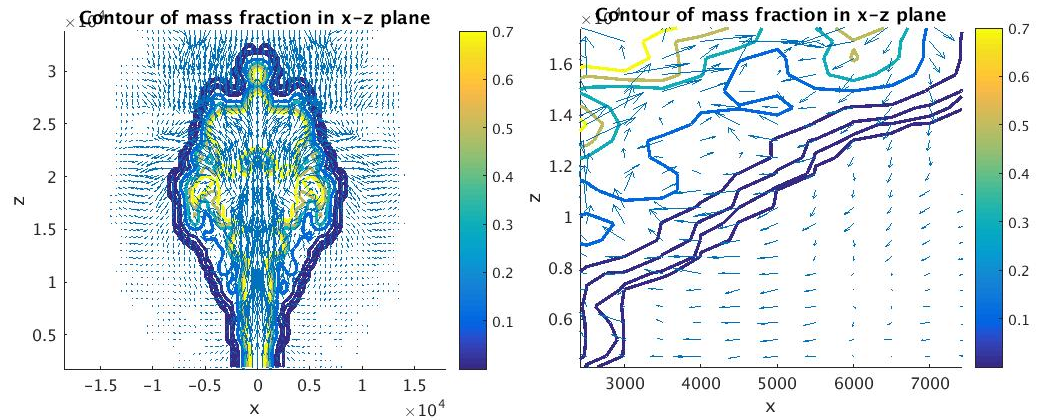
\includegraphics[width=10cm]{t100}
\caption{Contour of mass fraction and velocity quiver at 100 seconds, it keeps rising up and entraining air. The entrainment of air is clearly shown in zoomed view}
\label{fig:strong_plume_t100}
}
\end{figure}
\begin{figure}
\center
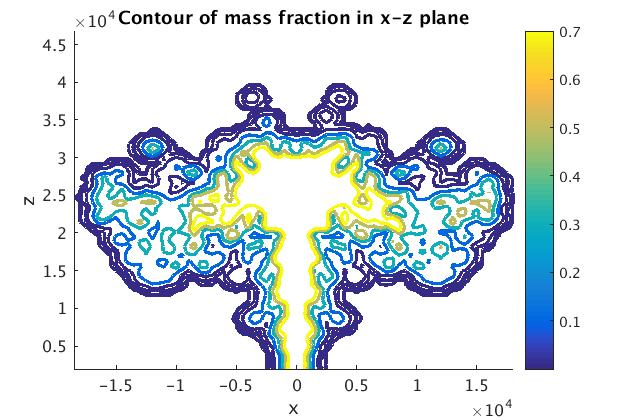
\includegraphics[width=5cm]{t200}
\caption{Contour of mass fraction at 200 seconds, plume reaches its top height}
\label{fig:strong_t200}
\end{figure}
\begin{figure}
\center
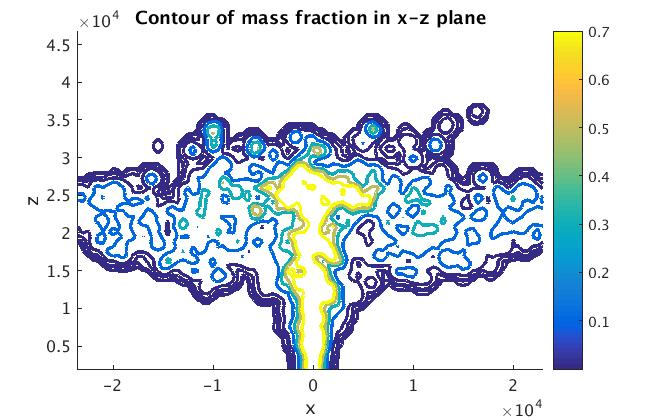
\includegraphics[width=5cm]{t300}
\caption{Contour of mass fraction at 300 seconds, the cloud is spreading}
\label{fig:strong_t300}
\end{figure}
Figure \ref{fig:strong_t15}~\ref{fig:strong_t300} shows the dynamic evolution process of volcano plume. The contour level of mass fraction are 0.7, 0.5, 0.3, 0.1, $1\times 10 ^{-1}$, $1\times 10 ^{-2}$, $1\times 10 ^{-3}$, $1\times 10^{-4}$ and $1\times 10^{-5}$. The plume keeps rising up and entraining air into the plume until it reaches its top height(around t=200 seconds). Afterwards the mixtures of erupted material and air then fall back to neutral height and starts spreading radially. Detailed velocity quiver plots show entraining of air into the plume at the edge of column. The evolution of the plume further verifies our model.
%
\conclusions  \label{sec:conclusion}%% \conclusions[modified heading if necessary]
A new plume model was developed based on SPH method. Advanced numerical techniques in SPH were exploited and tailored for this model. High performance computing was used to mitigate confliction between accuracy (depends on comprehensiveness of the model, resolution, order of accuracy of numerical methods, scheme for time upgrading.) and simulation time (depends on, comprehensiveness, resolution, order of accuracy of numerical methods, scheme for time upgrading ... and computational techniques). The correctness of the code and model was verified and validated by a series of test simulations.\\
Currently existing 3D models focus on certain aspect of the volcano plume (PDAC on pyroclastic flow, ATHAM on microphysics, and SK-3D on entrainment with higher accuracy and higher order of accuracy) and hence, naturally, different assumptions were made in these models. However, these different aspects of volcano plume are not independent and actually are coupled. In addition, there is no absolute boundary to determine which kind of hazard is dominant in certain eruption. So it is necessary to simulate all associated hazards in one model. Actually, effort has already been put on developing more comprehensive plume models. For example, a large-particle module (LPM) was added to ATHAM to track the paths of rocky particles (pyroclastic or tephra) within the plume and predicts where these particles fall \citep{kobs2009modeling}. We were also motivated by such a tendency of plume modeling to choose SPH as our numerical tool besides its ability in dealing with interface for multiple phase flows. As mentioned in the introduction section, SPH method has good extension features and adding of new physics and phases requires tiny modification on the code compared with mesh-based methods. The last but not the least, the dramatic development of computational power makes it possible to establish a comprehensive model. Even though right now, current computational capacity does not allow us to have too comprehensive model, the easy-extension feature of SPH makes it feasible to keep adding new physics into the model when necessary. What presented in this paper is actually our initial effort and results towards developing a first principle based plume model with comprehensive physics, adopting proper numerical tools and power of high performance computing. More advanced numerical techniques, such as adaptive particle size, Godnuv-SPH, semi-explicit time advancing scheme and better data management strategies and algorithms are on our list to exploit. In the near future, affect of wind field will be take into account. 
%In all existing 3D plume models, numerical calculations are performed on a non-uniform (vertically and horizontally stretched) grid, with different grid resolutions and domain sizes. However, implementation of different resolution in SPH methods is not straight forward and requires more work.
\section{Code availability}
The Plume-SPH code with a user manual providing instructions for installation, running and visualization are archived in github (https://github.com/Plume-SPH/plume-sph.git). The input data for all simulations presented in this work can also be found in the repository.
\section{Data availability}
Data for running the test cases, including meteorological data, properties of erupted material and air, and eruption condition data can be found in source code repository. Raw data of simulation results are archived in google drive. Access permission will be given upon request. Post-processed data for plotting figures is provided as supplement along with the manuscript. Please note that some of these pictures are generated by visualizing the raw data with visualization tools, there is no separate data for these figures.
%\appendix
%\section{}    %% Appendix A
%
%\subsection{}     %% Appendix A1, A2, etc.
%
%\appendixfigures  %% needs to be added in front of appendix figures in one-column style (\documentclass[acp, manuscript]{copernicus})
%
%\appendixtables   %% needs to be added in front of appendix tables in one-column style (\documentclass[acp, manuscript]{copernicus})
\authorcontribution{TEXT}
\competinginterests{Authors have the standard conflict with employers and listed sponsors}
%\disclaimer{TEXT}
\begin{acknowledgements}
All developers of Titan-2D, especially Dinesh Kumar who developed the GSPH version of Titan-2D, are greatly appreciated as Plume-SPH is based on their code. Advice and data (which is not shown in this paper) provided by Suzuki Yujiro gave us great help at the initial stage of model establishment and therefor are greatly appreciated. We appreciate Tomaso Esposti Ongaro for providing simulation data of PDAC (were also provided by Antonio Costa later together with other data) which helped us in doing early verification and improvement. We appreciate Antonio Costa for providing simulation results of existing 3D models, which are used in verification and validation section of this paper. We thank Matteo Cerminara for his helping on post-processing of plume simulation results. Computational results reported here were performed at the Center for Computational Research at the University at Buffalo. This project is supported by Grants No. NSF 1131074 from the National Science Foundation.
\end{acknowledgements}
%% REFERENCES
%% The reference list is compiled as follows:
\bibliographystyle{copernicus}
\bibliography{Reference.bib}
%% Since the Copernicus LaTeX package includes the BibTeX style file copernicus.bst,
%% authors experienced with BibTeX only have to include the following two lines:
%%
%% \bibliographystyle{copernicus}
%% \bibliography{example.bib}
%%
%% URLs and DOIs can be entered in your BibTeX file as:
%%
%% URL = {http://www.xyz.org/~jones/idx_g.htm}
%% DOI = {10.5194/xyz}
%% LITERATURE CITATIONS
%%
%% command                        & example result
%% \citet{jones90}|               & Jones et al. (1990)
%% \citep{jones90}|               & (Jones et al., 1990)
%% \citep{jones90,jones93}|       & (Jones et al., 1990, 1993)
%% \citep[p.~32]{jones90}|        & (Jones et al., 1990, p.~32)
%% \citep[e.g.,][]{jones90}|      & (e.g., Jones et al., 1990)
%% \citep[e.g.,][p.~32]{jones90}| & (e.g., Jones et al., 1990, p.~32)
%% \citeauthor{jones90}|          & Jones et al.
%% \citeyear{jones90}|            & 1990
%% FIGURES
%% When figures and tables are placed at the end of the MS (article in one-column style), please add \clearpage
%% between bibliography and first table and/or figure as well as between each table and/or figure.
%% ONE-COLUMN FIGURES
%%f
%\begin{figure}[t]
%\includegraphics[width=8.3cm]{FILE NAME}
%\caption{TEXT}
%\end{figure}
%
%%% TWO-COLUMN FIGURES
%
%%f
%\begin{figure*}[t]
%\includegraphics[width=12cm]{FILE NAME}
%\caption{TEXT}
%\end{figure*}
%
%
%%% TABLES
%%%
%%% The different columns must be seperated with a & command and should
%%% end with \\ to identify the column brake.
%
%%% ONE-COLUMN TABLE
%
%%t
%\begin{table}[t]
%\caption{TEXT}
%\begin{tabular}{column = lcr}
%\tophline
%
%\middlehline
%
%\bottomhline
%\end{tabular}
%\belowtable{} % Table Footnotes
%\end{table}
%
%%% TWO-COLUMN TABLE
%
%%t
%\begin{table*}[t]
%\caption{TEXT}
%\begin{tabular}{column = lcr}
%\tophline
%
%\middlehline
%
%\bottomhline
%\end{tabular}
%\belowtable{} % Table Footnotes
%\end{table*}
%
%
%%% MATHEMATICAL EXPRESSIONS
%
%%% All papers typeset by Copernicus Publications follow the math typesetting regulations
%%% given by the IUPAC Green Book (IUPAC: Quantities, Units and Symbols in Physical Chemistry,
%%% 2nd Edn., Blackwell Science, available at: http://old.iupac.org/publications/books/gbook/green_book_2ed.pdf, 1993).
%%%
%%% Physical quantities/variables are typeset in italic font (t for time, T for Temperature)
%%% Indices which are not defined are typeset in italic font (x, y, z, a, b, c)
%%% Items/objects which are defined are typeset in roman font (Car A, Car B)
%%% Descriptions/specifications which are defined by itself are typeset in roman font (abs, rel, ref, tot, net, ice)
%%% Abbreviations from 2 letters are typeset in roman font (RH, LAI)
%%% Vectors are identified in bold italic font using \vec{x}
%%% Matrices are identified in bold roman font
%%% Multiplication signs are typeset using the LaTeX commands \times (for vector products, grids, and exponential notations) or \cdot
%%% The character * should not be applied as mutliplication sign
%
%
%%% EQUATIONS
%
%%% Single-row equation
%
%\begin{equation}
%
%\end{equation}
%
%%% Multiline equation
%
%\begin{align}
%& 3 + 5 = 8\\
%& 3 + 5 = 8\\
%& 3 + 5 = 8
%\end{align}
%
%
%%% MATRICES
%
%\begin{matrix}
%x & y & z\\
%x & y & z\\
%x & y & z\\
%\end{matrix}
%
%
%%% ALGORITHM
%
%\begin{algorithm}
%\caption{_}
%\label{a1}
%\begin{algorithmic}
%_
%\end{algorithmic}
%\end{algorithm}
%
%
%%% CHEMICAL FORMULAS AND REACTIONS
%
%%% For formulas embedded in the text, please use \chem{}
%
%%% The reaction environment creates labels including the letter R, i.e. (R1), (R2), etc.
%
%\begin{reaction}
%%% \rightarrow should be used for normal (one-way) chemical reactions
%%% \rightleftharpoons should be used for equilibria
%%% \leftrightarrow should be used for resonance structures
%\end{reaction}
%
%
%%% PHYSICAL UNITS
%%%
%%% Please use \unit{} and apply the exponential notation
\end{document}
